% report = normales Tex-package
% scrreprt = koma-script package
\documentclass[pdftex, a4paper,11pt]{scrreprt}
% Glossar erstellen
\usepackage{glossary}
\makeglossary
% deutsche Silbentrennung
\usepackage[ngerman]{babel}
% wegen deutschen Umlauten
\usepackage[ansinew]{inputenc}
% Grafikpaket
\usepackage{graphicx}
\usepackage[bottom, hang]{footmisc}	% Zeilenumbr�che in Fu�noten verbessern
% Abstaende festlegen
\frenchspacing
%Font/Gr��e der �berschriften festlegen
\setkomafont{sectioning}{\normalcolor\bfseries}

% Begriffserk�rung
\usepackage{nomencl}
% Kommando umbenennen
\let\abbrev\nomenclature
% Deutsche �berschrift /Keine �berschrift
\renewcommand{\nomname}{Begriffserkl�rung}
% Zeilenabst�nde verkleinern
\setlength{\nomitemsep}{-\parsep}
\setlength{\nomlabelwidth}{.25\hsize}
\makenomenclature

\newcommand{\autor}{Philipp Rollwage, Christian Lins, Kai Ritterbusch, Andreas Depping}
\newcommand{\thema}{Software-Entwicklung im Bereich Projektmanagement}
\newcommand{\titel}{PrakMan: Der Praktikums-Manager}
\newcommand{\keywords}{Software-Engineering, PrakMan, Hausarbeit}

\newcommand{\gfxwidth}{1.0\textwidth}
\newcommand{\screensize}{0.4}

% PDF-Links erstellen
\usepackage[
	colorlinks	=true,
	linkcolor	=black, %blue,
	citecolor	=black, %blue,
	a4paper		=true,
	plainpages	=false,
	pdftex		=true,
	hyperindex	=true,
	pagebackref	=true,
	breaklinks	=true,
	bookmarks	=true,
	%bookmarksopen		=true,
	bookmarksnumbered	=true,
	pdfauthor	={\autor},
	pdftitle	={\titel},
	pdfkeywords	={\keywords},
	pdfsubject	={\thema},
	pdfcreator	={LaTeX},
	pdfproducer	={pdfTeX + hyperRef}
	%pdfmenubar=false,
	%pdftoolbar=false
]{hyperref}
\pdfcompresslevel =9

\date{\today}
\author{Philipp Rollwage \and Christian Lins \and Kai Ritterbusch \and Andreas Depping}
\title{\titel}

\begin{document}

\maketitle
\label{cha:Inhaltsverzeichnis}
\tableofcontents

%Kapitel der Ausarbeitung
\chapter{Programmkenndaten}
\label{cha:Programmkenndaten}

\section{Programmname}
\label{sec:Programmname}
Das Programm tr�gt den Namen seiner Funktionsbestimmung: Praktikumsmanager, abgek�rzt ``PrakMan''.

\section{Versionsnummer und Freigabedatum}
\label{sec:Version}
Das Programm liegt aktuell in der Version 1.0 vor und ist seit dem 17.09.2007 zur Nutzung freigegeben.

\section{Mitarbeiter}
\label{sec:Bearbeiter}
Mitarbeiter, die zu gleichen Teilen zur Fertigstellung der aktuell vorliegenden Version beigetragen haben sind:

\begin{itemize}
\item Andreas Depping \hfill Andreas.Depping@fh-osnabrueck.de\\
Bramscher Stra�e 158 \hfill Telefon: 0541/98252103\\
49088 Osnabr�ck \hfill Mat-Nr. \#325677
\item Christian Lins \hfill Christian.Lins@fh-osnabrueck.de\\
Limberger Stra�e 102 \hfill Telefon: 0541/3342152\\
49080 Osnabr�ck \hfill Mat-Nr. \#322141
\item Kai Ritterbusch \hfill Kai.Ritterbusch@fh-osnabrueck.de\\
Beethovenstra�e 8 \hfill Telefon: 05406/819606\\
49191 Belm \hfill Mat-Nr. \#327879
\item Philipp Rollwage \hfill Philipp.Rollwage@fh-osnabrueck.de\\
Neulandstra�e 6 \hfill Telefon: 0541/3247040\\
49084 Osnabr�ck \hfill Mat-Nr. \#329302
\end{itemize}

% 1.4. Aufgabenbeschreibung / Pflichtenheft
\section{Pflichtenheft}
\label{sec:Pflichtenheft}
Pflichtenheft zur Erstellung einer Software zur Praktikaverwaltung.
Das Projekt Praktika-Verwaltung beinhaltet die Planung und Realisierung eines Java-Programmsystems zur Verwaltung von Lehrveranstaltungen an der FH Osnabr�ck.

\subsection{Zielbestimmung}
\label{subsec:Zielbestimmung}
Es sollen Praktika (zum Beispiel zur Lehrveranstaltung Software Engineering) verwaltet werden. Dazu ist es notwendig, ca. 60 Studierende mit Hilfe einer GUI zu erfassen, in Praktikumsgruppen zu jeweils ca. 20 aufzuteilen und deren Anwesenheit in einer der ca. 15 Veranstaltungen im Semester zu erfassen.
Au�erdem sollen die Studierenden Projekten zugeordnet werden k�nnen. Dazu m�ssen ca. 6 Projekte zum Teil mehrfach angelegt werden k�nnen, denen jeweils ca. 1-8 Studierende zugeordnet werden.
Au�erdem sollen den Studierenden Hausarbeiten zugeordnet werden k�nnen. Dazu m�ssen ca. 4-8 Hausarbeiten zum Teil mehrfach angelegt werden k�nnen, denen jeweils ca. 1-8 Studierende zugeordnet werden.
Die Anwendung soll unterschiedliche Listen in unterschiedlicher Sortierung drucken k�nnen:
\begin{itemize}
\item Gesamtliste aller Studierenden der Veranstaltung
\item Liste der Studierenden je Praktikum
\item Liste mit Anwesenheit (gesamt und je Praktikum)
\item Notenlisten (``bestanden'' f�r Projekt, Note f�r Hausarbeit)
\end{itemize}

Das Programm muss �ber eine persistente Datenhaltung verf�gen, d.h. die Daten m�ssen in einer Datenbank oder in CSV-Dateien gehalten werden k�nnen.
Die CSV-Dateien sollen mit Excel eingelesen werden k�nnen.
Von jedem Studierenden werden die �blichen Daten erfasst (Name, Mat.-Nr, Semester, Studiengang, Email). W�nschenswert w�re eine Daten�bernahme aus den von StudIP exportierten Teilnehmerdaten.
Insgesamt soll eine benutzerfreundliche und leicht erweiterbare Anwendung zur Unterst�tzung von Lehrenden entstehen.

\subsubsection{Musskriterien}
\label{subsubsec:Musskriterien}
\begin{itemize}
\item Drucken von Anwesenheitslisten, Notenlisten
\item Wechsel von Studierenden zwischen Praktika
\item M�glichkeit, Studierende aus Praktika zu entfernen
\item Sortierungen nach unterschiedlichen Kriterien
\end{itemize}

\subsubsection{Wunschkriterien}
\label{subsubsec:Wunschkriterien}
\begin{itemize}
\item Schnittstelle zu StudIP: Import der dort exportierten Teilnehmerdaten
\item Verwaltung eines Fotos je Teilnehmer
%\item Filtern von Objekten
%\item Druckvorschau
\end{itemize}

\subsubsection{Abgrenzungskriterien}
\label{subsubsec:Abgrenzungskriterien} 
\begin{itemize}
\item Das Programm stellt keinen Ersatz f�r StudIP dar, sondern eine Unterst�tzung.
\item Es soll keine direkte Anbindung an die StudIP-Datenbank geben.
\end{itemize}

\subsection{Produkteinsatz}
\label{subsec:Produkteinsatz}
Das Programm soll von Professoren oder Tutoren, welche mit der Leitung von Praktikumsgruppen betraut sind, genutzt werden.

\subsubsection{Anwendungsbereiche}
\label{subsubsec:Anwendungsbereiche}
Das Programm soll es Professoren bzw. Tutoren erleichtern, ihre Praktikumsgruppen einzuteilen, Aufgaben und Noten zu verteilen und auf all diese Informationen in einer �bersichtlichen Oberfl�che zugreifen zu k�nnen.
Zur Haltung der Daten kann dabei eine eigene, lokale Datenbank genutzt werden, oder auch eine externe, auf die mehrere Tutoren mit ``PrakMan'' zugreifen und gemeinsam ihre Daten verwalten.

\subsubsection{Zielgruppen}
\label{subsubsec:Zielgruppen}
Das Programm soll von Professoren oder wissenschaftlichen Mitarbeitern, prim�r der Fachhochschule Osnabr�ck, eingesetzt werden. M�glich w�re aber auch ein Betrieb in anderen Hochschulen.
Vorausgesetzt werden grobe Kenntnisse im Bereich von Datenbanken (Zugangsdaten) oder Allgemeinwissen �ber Programme (M�gliche Optionen �ber Rechtsklick erreichbar etc.).

\subsubsection{Betriebsbedingungen}
\label{subsubsec:Betriebsbedingungen}
Das Programm ben�tigt keine gesonderte Beaufsichtigung, sondern kann direkt auf jedem PC, der die auf Seite \pageref{sec:Anforderungen} genannten Voraussetzungen erf�llt, genutzt werden.

\subsubsection{Software}
\label{subsubsec:Software}
Siehe Punkt \ref{sec:Anforderungen} auf Seite \pageref{sec:Anforderungen}.

\subsubsection{Hardware}
\label{subsubsec:Hardware}
Das Programm erfordert keine besondere Hardware.

\subsubsection{Orgware}
\label{subsubsec:Orgware}
Um den zu organisierenden Veranstaltungen Studenten hinzuf�gen zu k�nnen, m�ssen Daten �ber diese bekannt sein. Dazu geh�ren die Matrikelnummer, Vorname, Nachname und eine E-Mail-Adresse. Diese Daten sollten im Voraus entweder auf Papier oder per CSV (f�r den Import) organisiert werden.

\subsection{Schnittstellen}
\label{subsec:Schnittstellen}
Das Programm bietet eine JDBC-Schnittstelle, �ber die unterschiedliche Datenbanken angebunden werden k�nnen. ``PrakMan'' unterst�tzt momentan HSQL und PostgreSQL.

\subsection{Produktfunktionen}
\label{subsec:Produktfunktionen}

\subsubsection{/F0001/Verbindung zur Datenbank}
\label{subsubsec:/F0001/}
\paragraph{Voraussetzung:}
Keine
\paragraph{Ablauf:}
\begin{enumerate}
\item Der Benutzer startet das Programm und w�hlt einen Datenbanktypen aus: Lokal (HSQL) oder PostgreSQL.
\end{enumerate}
\paragraph{Alternativen:}
\begin{enumerate}
\item[1a.] Die Verbindung schl�gt fehl. Das kann an einer nicht vorhandenen Internetverbindung oder einem nicht gestarteten Datenbank-Server liegen.
\end{enumerate}

\subsubsection{/F0002/Erstellen einer Veranstaltung}
\label{subsubsec:/F0002/}
\paragraph{Voraussetzung:}
\begin{enumerate}
\item Der Benutzer hat PrakMan gestartet und die Verbindung zu einer Datenbank erfolgreich hergestellt.
\end{enumerate}
\paragraph{Ablauf:}
\begin{enumerate}
\item Der Benutzer klickt im Baum mit der rechten Maustaste auf den Ast ``Veranstaltungen'' und w�hlt ``Hinzuf�gen'' aus.
\item Ein Professor wird ausgew�hlt, der die Veranstaltung betreuen soll.
\item Die neue Veranstaltung ist erstellt, nun k�nnen weitere Einstellungen getroffen werden. 
\end{enumerate}
\paragraph{Alternativen:}
\begin{enumerate}
\item[1a.] Ein Datenbankfehler tritt auf. Die Verbindung zur Datenbank sollte �berpr�ft werden.
\end{enumerate}

\subsubsection{/F0003/Hinzuf�gen von Studenten zu einer Veranstaltung}
\label{subsubsec:/F0003/}
\paragraph{Voraussetzung:}
\begin{enumerate}
\item Der Benutzer hat PrakMan gestartet und die Verbindung zu einer Datenbank erfolgreich hergestellt.
\item Es existiert mindestens eine Veranstaltung.
\end{enumerate}
\paragraph{Ablauf:}
\begin{enumerate}
\item Der Benutzer �ffnet die Ansicht der Veranstaltung �ber einen Doppelklick auf Selbige.
\item �ber den Plus-Button am unteren Rand des Fensters wird ein neues Panel ge�ffnet, �ber welches Studenten ausgew�hlt und durch einen Druck auf ``Ok'' der Veranstaltung hinzugef�gt werden.
\end{enumerate}
\paragraph{Alternativen:}
\begin{enumerate}
\item[2a.] Es existieren keine Studenten. In diesem Fall m�ssen erst neue Studenten manuell erstellt oder �ber CSV eingelesen werden.
\end{enumerate} 

\subsubsection{/F0004/Einteilung der Studenten in Gruppen}
\label{subsubsec:/F0004/}
\paragraph{Voraussetzung:}
\begin{enumerate}
\item Der Benutzer hat PrakMan gestartet und die Verbindung zu einer Datenbank erfolgreich hergestellt.
\item Es existiert mindestens eine Veranstaltung, deren Gruppen-Ansicht ge�ffnet ist.
\end{enumerate}
\paragraph{Ablauf:}
\begin{enumerate}
\item Ein Klick auf den Plus-Button erstellt eine neue Gruppe. �ber einen Doppelklick auf ihren Namen kann deren Beschreibung editiert werden.
\item Der Benutzer wechselt in die Teilnehmer-Ansicht und markiert dort �ber einfaches Ziehen mit der Maus, oder Shift/Strg-Klick einen oder mehrere Studenten, die zusammen eine Gruppe bilden sollen. �ber einen rechtsklick auf die Tabelle kann diesen markierten Studenten nun eine Gruppe zugewiesen werden.
\end{enumerate}
\paragraph{Alternativen:}
\begin{enumerate}
\item[1a.] Ein Datenbankfehler tritt auf. Die Verbindung zur Datenbank sollte �berpr�ft werden.
\item[2a.] Es existieren noch keine Studenten in der Veranstaltung. In diesem Fall, k�nnen sie einfach �ber den Plus-Button in der Teilnehmer-Ansicht hinzugef�gt werden.
\end{enumerate}

\subsubsection{/F0005/Ein Projekt hinzuf�gen}
\label{subsubsec:/F0005/}
\paragraph{Voraussetzung:}
\begin{enumerate}
\item Der Benutzer hat PrakMan gestartet und die Verbindung zu einer Datenbank erfolgreich hergestellt.
\item Es existiert mindestens eine Veranstaltung, deren Projekte-Ansicht ge�ffnet ist.
\end{enumerate}
\paragraph{Ablauf:}
\begin{enumerate}
\item Ein Klick auf den Plus-Button erstellt ein neues unbenanntes Projekt.
\item �ber einen Doppelklick auf Selbiges, k�nnen diesem Projekt Teilnehmer hinzugef�gt und au�erdem dessen Beschreibung editiert werden. Zus�tzlich kann eine ``Deadline'' gesetzt werden, zu welcher dieses Projekt beendet sein muss.
\end{enumerate}
\paragraph{Alternativen:}
\begin{enumerate}
\item[1a.] Ein Datenbankfehler tritt auf. Die Verbindung zur Datenbank sollte �berpr�ft werden.
\item[2a.] Es existieren keine Studenten, die zugeordnet werden k�nnen. In diesem Fall, k�nnen sie einfach �ber den Plus-Button in der Teilnehmer-Ansicht hinzugef�gt werden.
\end{enumerate}

\subsubsection{/F0006/Einen Termin hinzuf�gen}
\label{subsubsec:/F0006/}
\paragraph{Voraussetzung:}
\begin{enumerate}
\item Der Benutzer hat PrakMan gestartet und die Verbindung zu einer Datenbank erfolgreich hergestellt.
\item Es existiert mindestens eine Veranstaltung, deren Termine-Ansicht ge�ffnet ist.
\end{enumerate}
\paragraph{Ablauf:}
\begin{enumerate}
\item Ein Klick auf den Plus-Button �ffnet ein Auswahlfenster, in dem ein Termin f�r die Veranstaltung ausgew�hlt werden kann. Zuerst sollte eine Uhrzeit angegeben werden. Ein Klick auf einen Tag im Kalender f�gt diesen Termin dann der Veranstaltung hinzu.
\end{enumerate}
\paragraph{Alternativen:} Keine

\subsubsection{/F0007/Den Tutor einer Veranstaltung �ndern}
\label{subsubsec:/F0007/}
\paragraph{Voraussetzung:}
\begin{enumerate}
\item Der Benutzer hat PrakMan gestartet und die Verbindung zu einer Datenbank erfolgreich hergestellt.
\item Es existiert mindestens eine Veranstaltung.
\end{enumerate}
\paragraph{Ablauf:}
\begin{enumerate}
\item �ber einen Doppelklick auf eine Veranstaltung links im Baum, �ffnet sich deren Hauptansicht. Nun kann �ber die Dropdown-Box im oberen rechten Bereich einer der in der Datenbank registrierten Professoren ausgew�hlt werden.
\item �ber den Button ``Speichern'' (oben links) wird die Information in die Datenbank �bernommen.
\end{enumerate}
\paragraph{Alternativen:}
\begin{enumerate}
\item[1a.] Statt einer Veranstaltung wird im Baum ein Lehrender ausgew�hlt. Bei diesem kann dann �ber den Plus-Button eine Veranstaltung zugeordnet werden.
\item[1b.] Es ist kein weiterer Professor vorhanden. In dem Fall m�ssen manuell oder per CSV-Import neue Lehrende hinzugef�gt werden.
\item[2a.] Ein Datenbankfehler tritt auf. Die Verbindung zur Datenbank sollte �berpr�ft werden.
\end{enumerate}

\subsubsection{/F0008/Einen neuen Dozenten hinzuf�gen}
\label{subsubsec:/F0008/}
\paragraph{Voraussetzung:}
\begin{enumerate}
\item Der Benutzer hat PrakMan gestartet und die Verbindung zu einer Datenbank erfolgreich hergestellt.
\end{enumerate}
\paragraph{Ablauf:}
\begin{enumerate}
\item Der Benutzer klickt im Baum mit der rechten Maustaste auf den Ast ``Lehrende'' und w�hlt ``Hinzuf�gen'' aus.
\item Im auftauchenden Panel werden die ben�tigten Daten ``Vorname'' und ``Nachname'' eingetragen.
\item Ein Druck auf den Button ``Speichern'' �bertr�gt die Informationen in die Datenbank, der neue Dozent ist erstellt.
\end{enumerate}
\paragraph{Alternativen:}
\begin{enumerate}
\item[3a.] Ein Datenbankfehler tritt auf. Die Verbindung zur Datenbank sollte �berpr�ft werden.
\end{enumerate}

\subsubsection{/F0009/Einen neuen Studenten hinzuf�gen}
\label{subsubsec:/F0009/}
\paragraph{Voraussetzung:}
\begin{enumerate}
\item Der Benutzer hat PrakMan gestartet und die Verbindung zu einer Datenbank erfolgreich hergestellt.
\end{enumerate}
\paragraph{Ablauf:}
\begin{enumerate}
\item Der Benutzer klickt im Baum mit der rechten Maustaste auf den Ast ``Studenten'' und w�hlt ``Hinzuf�gen'' aus.
\item Im auftauchenden Eingabefeld wird die 6-stellige Matrikelnummer des Studenten angegeben. Ein Druck auf ``OK'' l�sst ein neues Panel erscheinen.
\item Im erschienenen Panel werden die ben�tigten Daten ``Vorname'', ``Nachname'' und ``E-Mail'' eingetragen.
\item Ein Druck auf den Button ``Speichern'' �bertr�gt die Informationen in die Datenbank, der neue Student ist erstellt.
\end{enumerate}
\paragraph{Alternativen:}
\begin{enumerate}
\item[4a.] Ein Datenbankfehler tritt auf. Die Verbindung zur Datenbank sollte �berpr�ft werden.
\end{enumerate}

\subsubsection{/F0010/Daten in CSV exportieren}
\label{subsubsec:/F0010/}
\paragraph{Voraussetzung:}
\begin{enumerate}
\item Der Benutzer hat PrakMan gestartet und die Verbindung zu einer Datenbank erfolgreich hergestellt.
\end{enumerate}
\paragraph{Ablauf:}
\begin{enumerate}
\item Der Benutzer klickt im Baum mit der rechten Maustaste auf einen der �ste ``Lehrende'', ``Studenten'' \emph{oder} direkt auf eine bestimmte Veranstaltung und w�hlt ``Export''.

Wird ein Ast ausgew�hlt, werden nur die Informationen der Objekte in diesem Ast in der CSV-Datei gespeichert. Wird eine einzelne Veranstaltung ausgew�hlt, werden deren gesamte Informationen detailliert gespeichert. Dies beinhaltet Gruppen, Aufgaben, Teilnehmer und Termine.
\item Der Benutzer w�hlt im auftauchenden Dialog einen Dateinamen. Ein Druck auf ``Speichern'' beendet die Aktion und erstellt die CSV-Datei mit den gew�nschten Informationen.
\end{enumerate}
\paragraph{Alternativen:}
\begin{enumerate}
\item[1a.] Es gibt noch keine Veranstaltungen, Lehrenden oder Studenten. In dem Fall wird auch nichts exportiert.
\item[2a.] Der Benutzer hat kein Schreibrecht, das Speichern schl�gt fehl. In diesem Fall sollten Sie Ihre Benutzerrechte auf dem PC �berpr�fen.
\end{enumerate} 

\subsubsection{/F0011/CSV-Daten importieren}
\label{subsubsec:/F0011/}
\paragraph{Voraussetzung:}
\begin{enumerate}
\item Der Benutzer hat PrakMan gestartet und die Verbindung zu einer Datenbank erfolgreich hergestellt.
\end{enumerate}
\paragraph{Ablauf:}
\begin{enumerate}
\item Der Benutzer klickt im Baum mit der rechten Maustaste auf einen der �ste ``Lehrende'', ``Studenten'' \emph{oder} direkt auf eine bestimmte Veranstaltung und w�hlt ``Import''.

Wird ein Ast ausgew�hlt werden nur Listeninformationen der Objekte in diesen Ast �bernommen. Wird eine einzelne Veranstaltung ausgew�hlt, wird auch eine CSV-Datei mit detaillierten Informationen �ber diese Veranstaltung ben�tigt. Dies beinhaltet Gruppen, Aufgaben, Teilnehmer und Termine.
\item Der Benutzer w�hlt im auftauchenden Dialog einen Dateinamen. Ein Druck auf ``�ffnen'' beendet die Aktion und erstellt die Objekte im Baum respektive f�llt die gew�hlte Veranstaltung mit detaillierten Informationen.
\end{enumerate}
\paragraph{Alternativen:}
\begin{enumerate}
\item[1a.] Es gibt noch keine Veranstaltung, die direkt ausgew�hlt werden kann. In diesem Fall m�ssen Sie zuerst eine Veranstaltung erstellen.
\item[2a.] Ihre CSV-Datei ist falsch formatiert und wird vom System nicht verstanden.
\end{enumerate}

\subsubsection{/F0012/Ein Projekt benoten}
\label{subsubsec:/F0012/}
\paragraph{Voraussetzung:}
\begin{enumerate}
\item Der Benutzer hat PrakMan gestartet und die Verbindung zu einer Datenbank erfolgreich hergestellt.
\item Es existiert mindestens eine Veranstaltung, die zumindest ein Projekt enth�lt und deren Projekte-Ansicht ge�ffnet ist.
\end{enumerate}
\paragraph{Ablauf:}
\begin{enumerate}
\item Ein Doppelklick auf das Projekt �ffnet ein Auswahlfenster, in dem Ausgabe -und Abgabetermin festgelegt, Studenten zum Projekt hinzugef�gt und dessen Beschreibung editiert werden kann.
\item Ein Doppelklick auf das Notenfeld eines Studenten �ffnet eine Eingabemaske, in der eine neue Note f�r diesen Studenten festgelegt werden kann.
\end{enumerate}
\paragraph{Alternativen:}
Keine


\subsection{Produktdaten}
\label{subsec:Produktdaten}

\subsubsection{/D0001/Studentendaten}
\label{subsubsec:/D0001/}
Vorname, Nachname, E-Mail-Adresse und Matrikelnummer von Studenten. Des weiteren Projekte und Termine, an denen Studenten teilnehmen bzw. teilgenommen haben sowie die Benotung einzelner Projekte.

\subsubsection{/D0002/Dozentendaten}
\label{subsubsec:/D0002/}
Vorname und Nachname eines Dozenten.

\subsubsection{/D0003/Veranstaltungsdaten}
\label{subsubsec:/D0003/}
Name, Beschreibung, Teilnehmer, Projekte und Termine einer Veranstaltung.

\subsection{Produktleistungen}
\label{subsec:Produktleistungen}

\subsubsection{/L0001/Komfort}
\label{subsubsec:/L0001/}
Das Erstellen von Veranstaltungen, F�llen mit Studenten und Verteilen von Aufgaben soll m�glichst einfach und schnell m�glich sein. Das Programm soll die Arbeit erleichtern und nicht verkomplizieren.

\subsection{Benutzungsoberfl�che}
\label{subsec:Benutzungsoberflaeche}

\subsubsection{Bildschirmlayout}
\label{subsubsec:Bildschirmlayout}
Das Bildschirmlayout soll die Daten �bersichtlich darstellen und einen m�glichst schnellen und effektiven Zugriff erm�glichen. Es soll m�glich sein, mehrere Informationen gleichzeitig zu �ffnen.

\subsubsection{Drucklayout}
\label{subsubsec:Drucklayout}
Das Drucklayout soll m�glichst �bersichtlich Informationen �ber die Teilnehmer einer Veranstaltung und deren Benotung liefern.

\subsubsection{Tastaturlayout}
\label{subsubsec:Tastaturlayout}
Eine gesonderte Hotkey-Nutzung der Tastatur ist nicht vorgesehen. Das Programm soll es daf�r erm�glichen, mit der Maus m�glichst einfach von einer Information zur n�chsten damit zusammenh�ngenden zu kommen.

\subsubsection{Dialoglayout}
\label{subsubsec:Dialoglayout}
Die Dialoge sollen m�glichst viele Icons enthalten, die ihren Zweck direkt deutlich machen. Dazu sollen Tooltips existieren, die auch bei einer Unklarheit weiterhelfen.

\subsection{Qualit�tszielbestimmungen}
\label{subsec:Qualitaetszielbestimmungen}
\begin{itemize}
\item Funktionalit�t: \hfill Sehr wichtig
\item Zuverl�ssigkeit: \hfill Wichtig
\item Benutzbarkeit: \hfill Relativ wichtig
\item Effizienz: \hfill Unwichtig
\item �bertragbarkeit: \hfill Vernachl�ssigbar
\end{itemize}

\subsection{Globale Testszenarien und Testf�lle}
\label{subsec:Testszenarien}

\subsubsection{/T0001/Eingabe einer bereits vorhandenen oder negativen Matrikel-Nr.}
\label{subsubsec:/T0001/}
Die Eingabe wird mit einer Fehlermeldung zur�ckgewiesen.

\subsubsection{/T0002/Angeben einer ung�ltig formatierten CSV-Datei beim Import}
\label{subsubsec:/T0002/}
Die Datei wird als falsch formatiert zur�ckgewiesen.


\subsection{Entwicklungsumgebung}
\label{subsec:Entwicklungsumgebung}
\begin{itemize}
\item Java 1.5
\item Eclipse
\item Subversion zur verbesserten Teamarbeit
\end{itemize}

\subsection{Erg�nzungen}
\label{subsec:Ergaenzungen}
Keine Erg�nzungen.

\subsection{Begriffserkl�rung}
\label{subsec:Begriffserklaerung}
Vollst�ndige Erkl�rung wichtiger Begriffe, siehe Abschnitt \ref{chap:Glossar} (S.\pageref{chap:Glossar}).


\section{L�sungsverfahren und Algorithmen}
\label{sec:Algorithmen}
Es werden keine au�ergew�hnlichen Algorithmen verwendet.

\section{Hardware- und Softwareanforderungen}
\label{sec:Anforderungen}
Zum Betrieb des Programms erforderlich sind
\begin{itemize}
\item Java Version 1.5 oder h�her
\item F�r Mehrbenutzer-Verwendung: Eine externe Datenbank (Postgres)
\item Bei lokaler Nutzung: Speicherplatz f�r die zu haltenden Daten
\end{itemize}

\section{Ben�tigte Dateien und Directories}
\label{sec:DateienUndDirectories}
Zum Start des Programms wird allein die Datei ``prakman.jar'' ben�tigt, welche das Programm sowie alle Treiber f�r die unterst�tzten Datenbanken enth�lt.

\chapter{Programmaufbau und Dokumentation}
\label{cha:ProgrammaufbauUndDokumentation}
% Programmstruktur mit Funktionsbaum, Gesch�ftsprozessen mit Strukturierter Analyse
% Datenflussdiagrammen ( DFD ) und Data Dictionary ( DD ), sowie Gliederung der
% Module/Packages und deren Klassen mit kurzer Leistungsbeschreibung

\section{Programmstruktur}
\label{sec:Programmstruktur}
Die folgenden Abschnitte pr�sentieren, oftmals in graphischer Form, den Aufbau sowie die Funktionsweise und den Fluss der Daten in ``PrakMan''.

\subsection{Datenflussdiagramm}
\label{subsec:Datenflussdiagramm}
S�mtliche Daten werden in ``PrakMan'' in einer Datenbank verwaltet. Alle Informationen gehen dort hinein und kommen von dort zur�ck. Diese verwaltet somit immer den aktuellen Stand der Informationen. Abbildung \ref{img:DFD} (S.\pageref{img:DFD}) veranschaulicht den Datenfluss in einem Diagramm.

\begin{figure}[hb]
\begin{center}
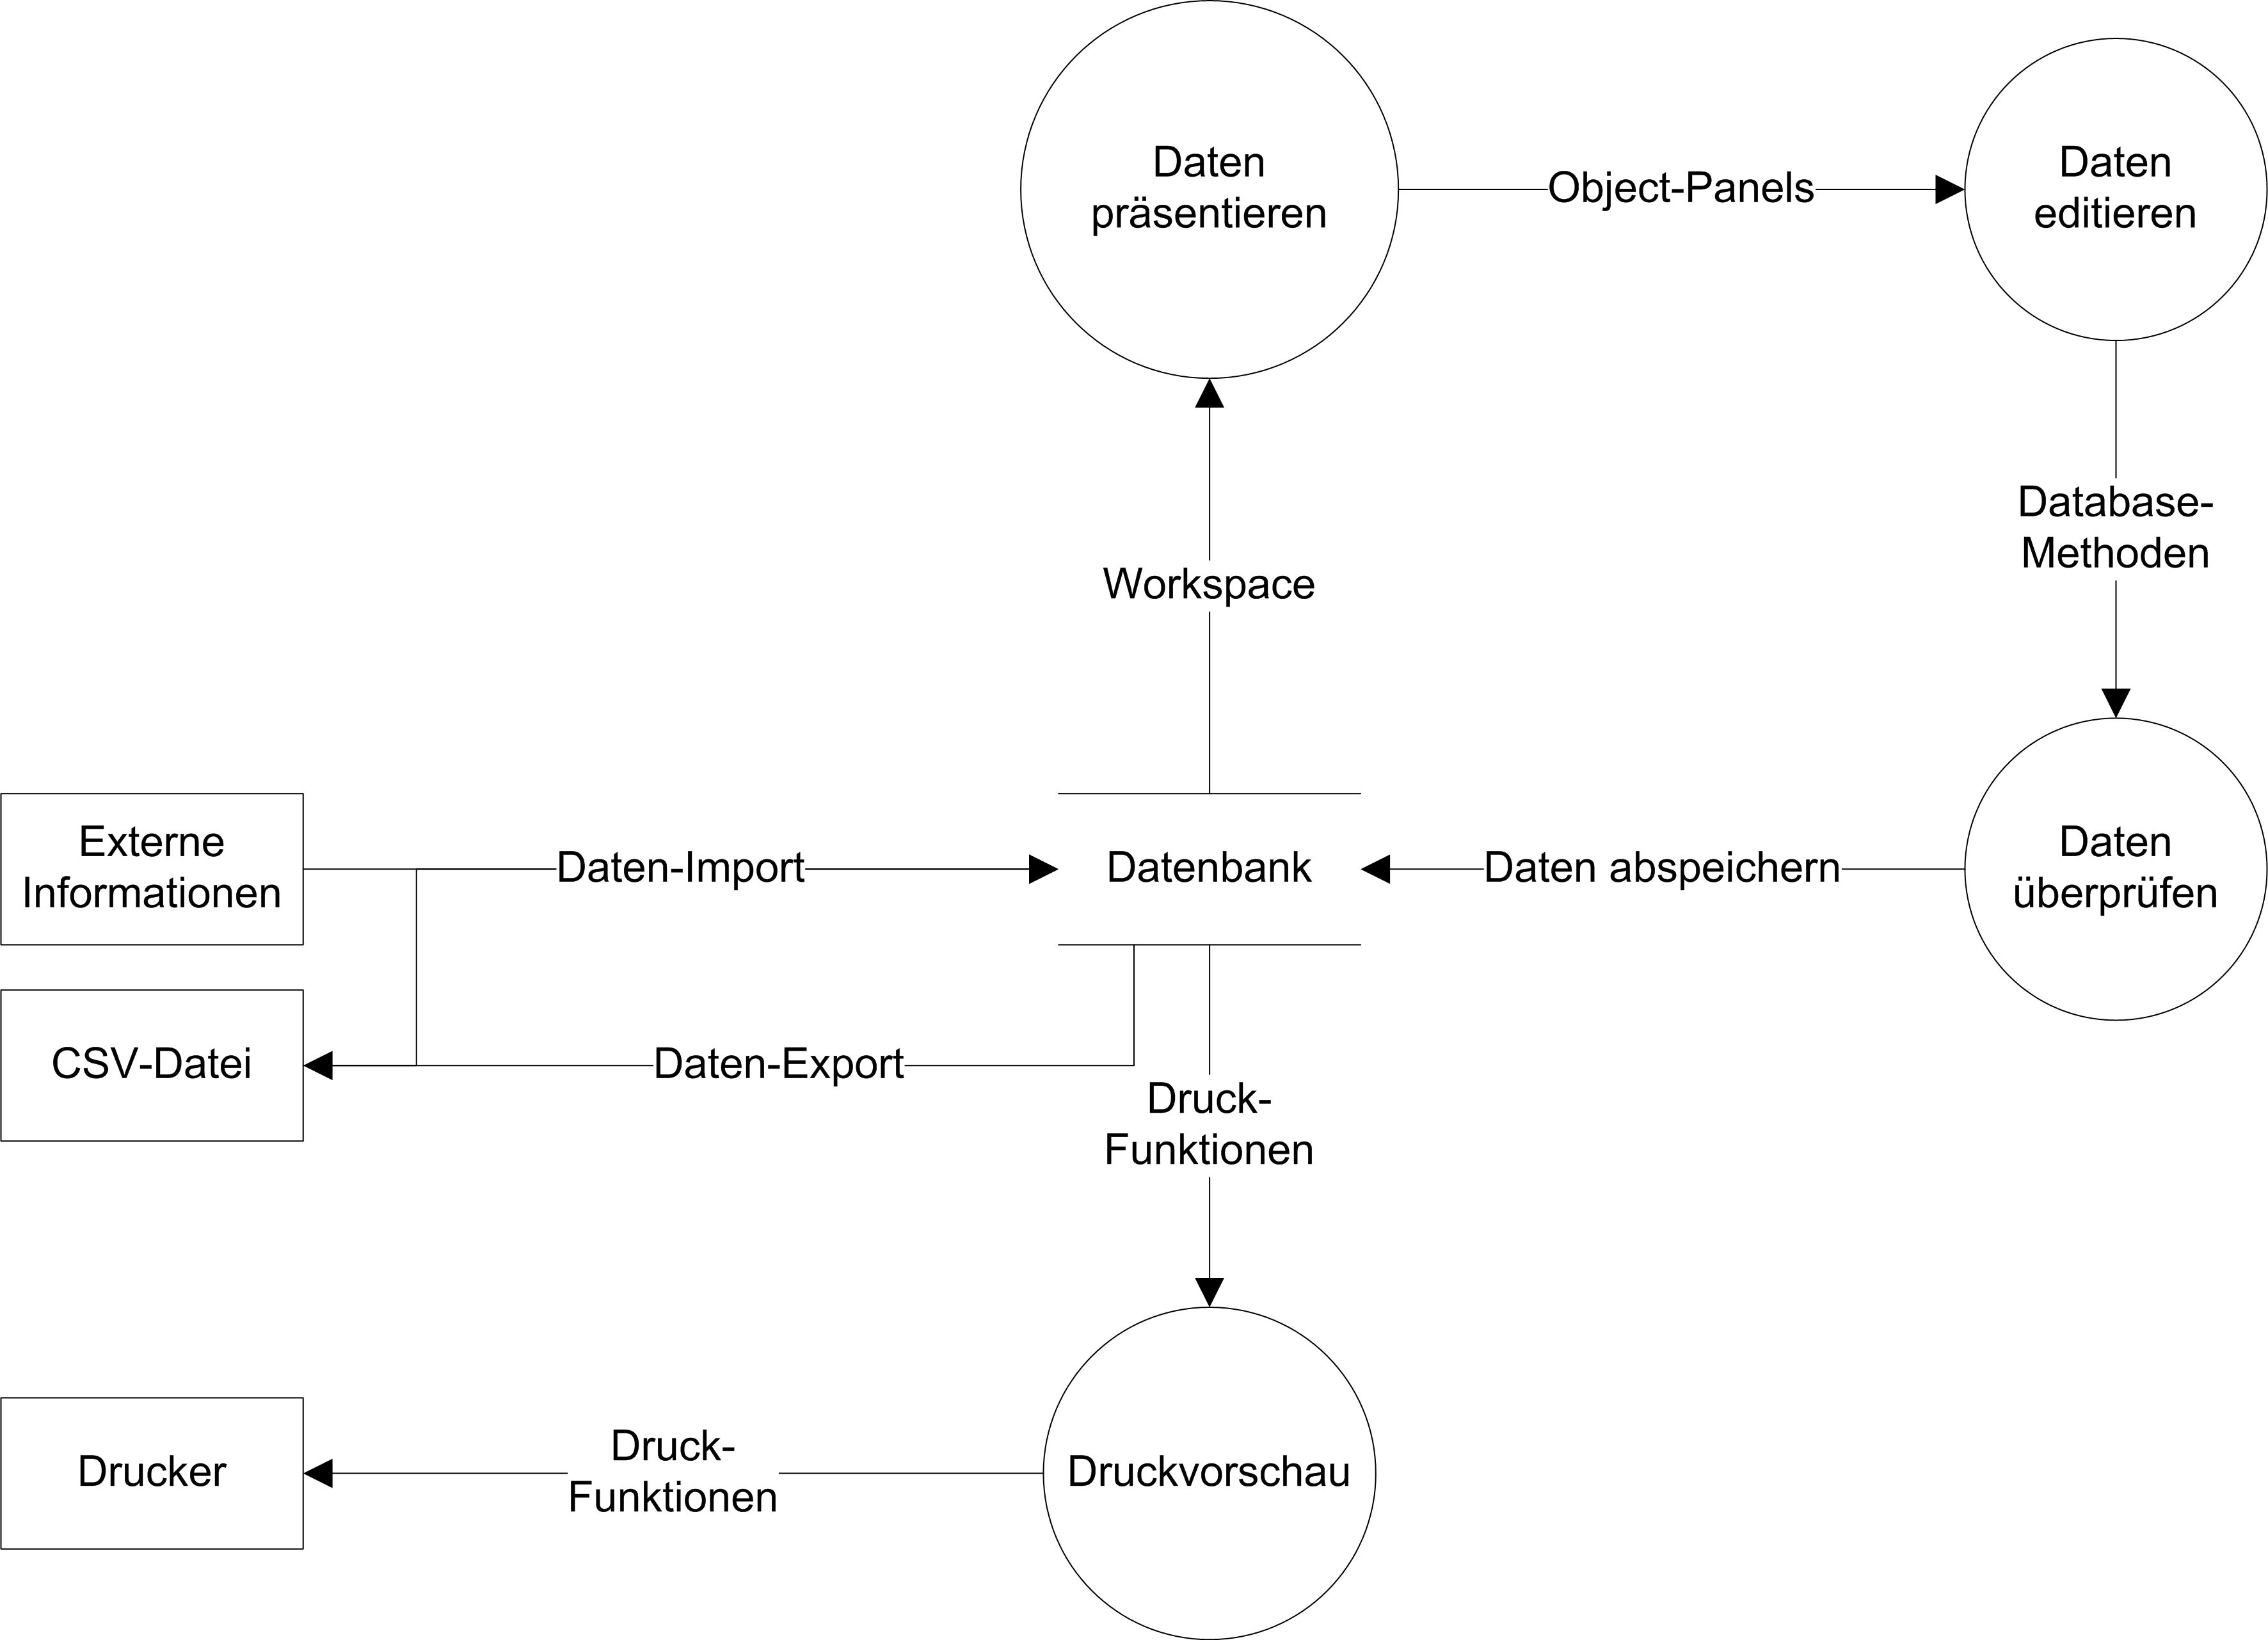
\includegraphics[width=\gfxwidth]{gfx/DFD}
\caption{Datenflussdiagramm von ``Prakman''}
\label{img:DFD}
\end{center}
\end{figure}

%\subsection{Funktionsbaum}
%\label{subsec:Funktionsbaum}

\subsection{Gliederung der Packages}
\label{subsec:GliederungDerPackages}
Abbildung \ref{img:Paketgliederung} (S.\pageref{img:Paketgliederung}) stellt die Gliederung der Pakete in ``PrakMan'' dar.
Das Grundpaket ist hierbei in hellblau dargestellt, darunter folgen unterschiedliche Farben f�r jeweils andere Bereiche. Die Farben sind je nach weiterer Spezialisierung des Pakets in steigender Intensit�t gew�hlt.

Hier ist - wie auch im Klassenhierarchiediagramm unter Punkt \ref{img:Klassenhierarchiediagramm} (S.\pageref{img:Klassenhierarchiediagramm}) - deutlich die Aufteilen von ``PrakMan'' zu erkennen:
\begin{itemize}
\item Das Paket ``prakman.io'' sorgt f�r den Informationsfluss. Es speichert die Daten in der Datenbank und stellt sie wiederum bereit.
\item Das Paket ``prakman.model'' stellt Objekte bereit, die die Informationen aus der Datenbank logisch kapseln und dann zur Weiterverarbeitung genutzt werden k�nnen.
\item Das Paket ``prakman.view'' stellt die Daten f�r den Benutzer dar, sorgt aber auch f�r die Interaktion mit dem Benutzer.
\item Das Paket ``resource'' ist lediglich ein Speicherort f�r Icons, k�nnte jedoch noch auf weitere Resourcen wie z.B. abgelegte Fotos etc. erweitert werden.
\end{itemize}

\begin{figure}[hb]
\begin{center}
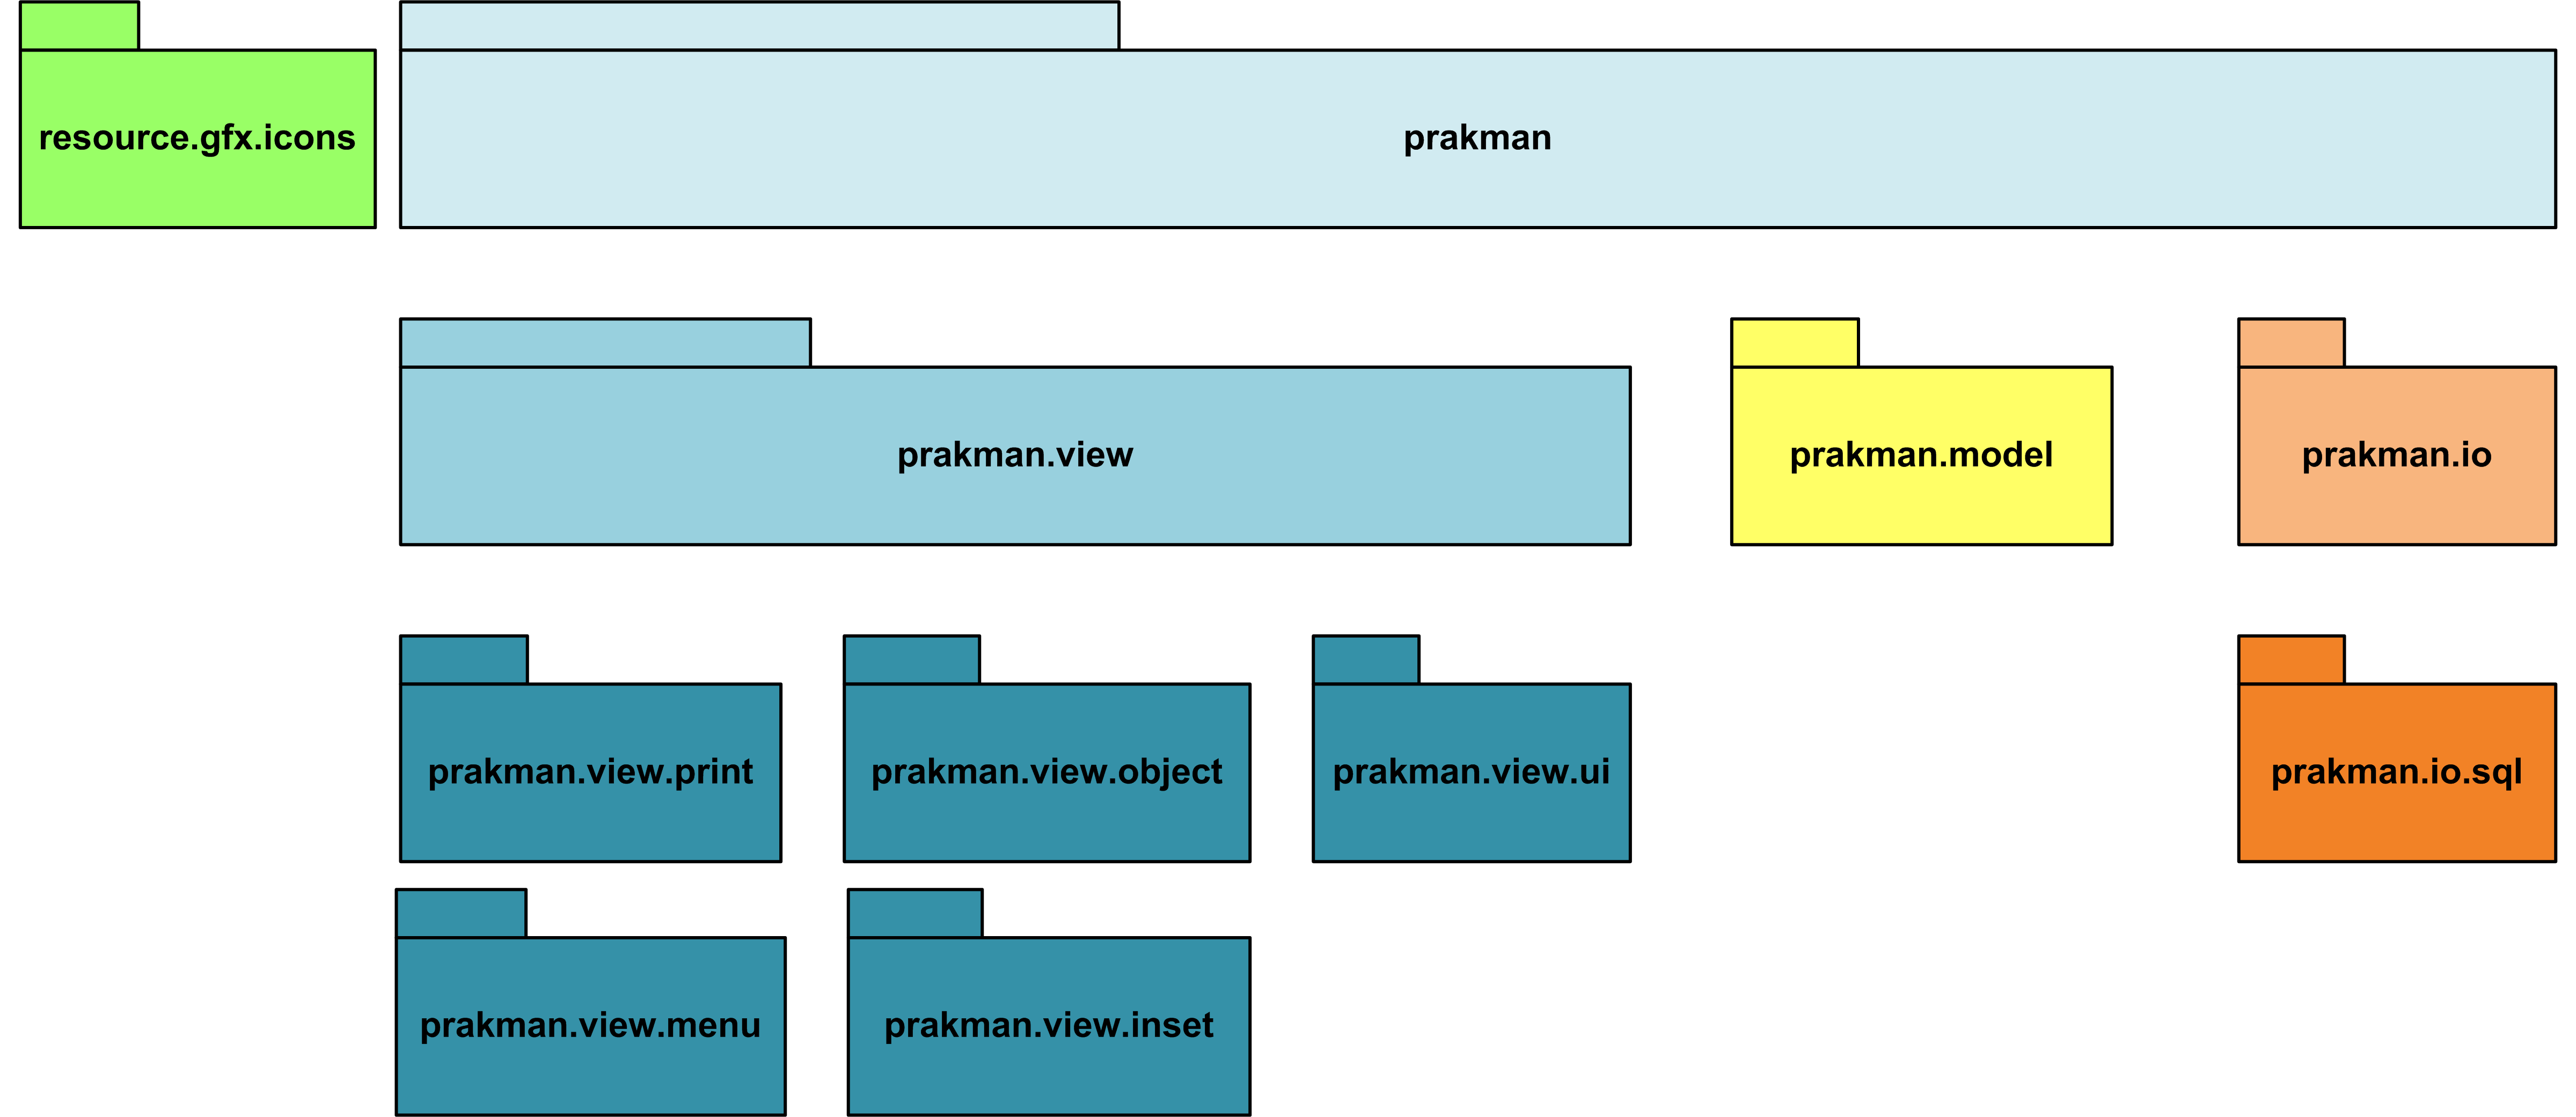
\includegraphics[width=\gfxwidth]{gfx/PaketGliederung}
\caption{Paketgliederung von ``Prakman''}
\label{img:Paketgliederung}
\end{center}
\end{figure}

\section{Klassenhierarchiediagramm} % in UML- Notation
\label{sec:Klassenhierarchiediagramm}
Abbildung \ref{img:Klassenhierarchiediagramm} (S.\pageref{img:Klassenhierarchiediagramm}) stellt die Schichtung des Programms und das Zusammenspiel der wichtigsten Klassen von ``PrakMan'' in Form eines Klassenhierarchiediagramms dar.
Hierbei befinden sich in der obersten Schicht die Klassen, welche die Darstellung �bernehmen. In der Schicht darunter folgen die Objekte, welche die Informationen aus der Datenbank in Objekten gekapselt pr�sentieren. Die daruner liegende Schicht enth�lt die Klassen, �ber die diese Informationen bezogen werden. Schlie�lich ist in der untersten Schicht zus�tzlich die Startklasse sowie eine Klasse, welche das Speichern von lokalen Konfigurationsdaten �bernimmt, dargestellt.

\begin{figure}[hb]
\begin{center}
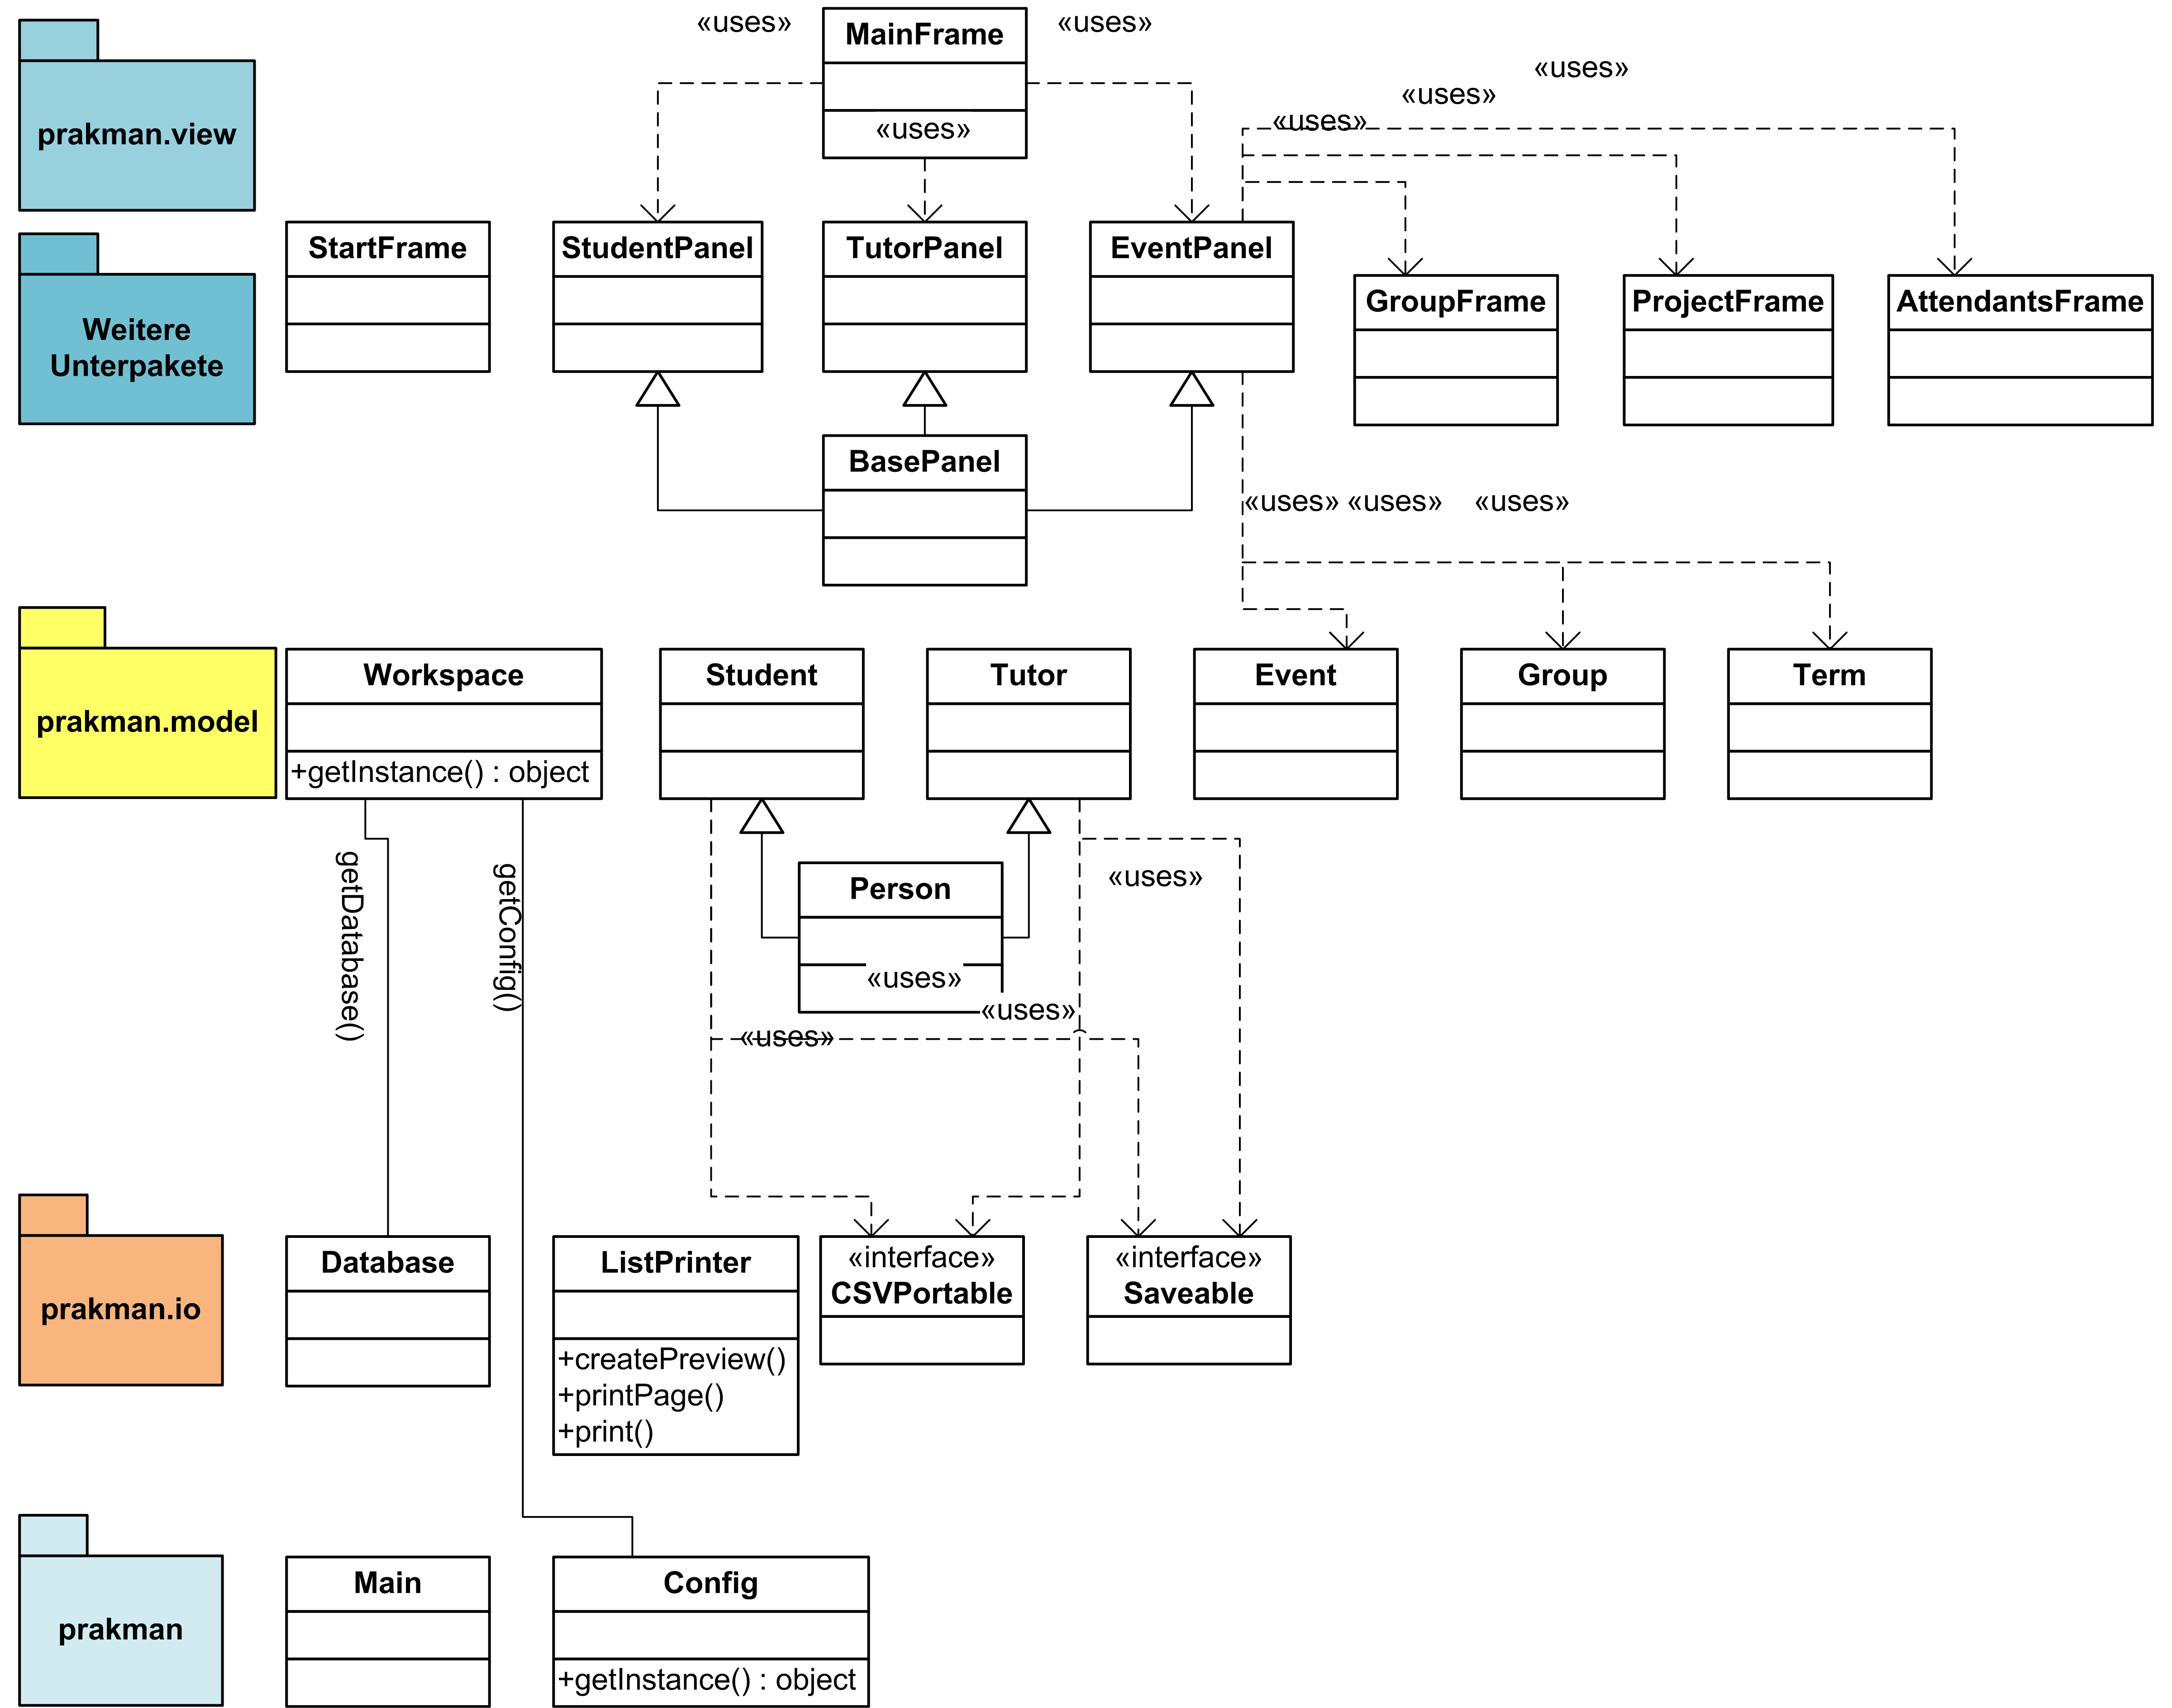
\includegraphics[width=\gfxwidth]{gfx/Klassendiagramm}
\caption{Klassenhierarchiediagramm von ``Prakman'' (wichtige Klassen)}
\label{img:Klassenhierarchiediagramm}
\end{center}
\end{figure}


\section{Klassendokumentation}
\label{sec:Klassendokumentation}
% mit Attributen und Operationen und deren vollst�ndiger
% Schnittstellenspezifikation mit Typdefinitionen, Parametern, Resultaten und
% Leistungsbeschreibung, sowie Fehlermeldungen . mittels javadoc
Siehe Verzeichnis ``Javadoc'' auf der beiliegenden CD.

%\section{Innere Dokumentation}
%\label{sec:InnereDokumentation}
% mit Leistungsbeschreibung, kommentierten Listings, Beschreibung
% der Parameter und Variablen, Kurz-/Lang- und JAVA- Kommentare


% experimentell
\clearpage

\section{Programmablauf}
\label{sec:Programmablauf}
% mit Struktogrammen, Programmablaufpl�nen, etc.
Die folgenden Programmablaufpl�ne verdeutlichen, wie die in Kapitel \ref{subsec:Produktfunktionen} (S.\pageref{subsec:Produktfunktionen}) geforderten Funktionen in der Praxis in ``PrakMan'' umgesetzt sind.

\paragraph{/F0001/Verbindung zur Datenbank:}
Die Planung der Funktion kann dem Pflichtenheft, Kapitel \ref{subsubsec:/F0004/} (S.\pageref{subsubsec:/F0004/}) entnommen werden. Die Umsetzung ist in der Abbildung \ref{img:Ablauf_start} (S.\pageref{img:Ablauf_start}) dargestellt.

\begin{figure}[hb]
\begin{center}
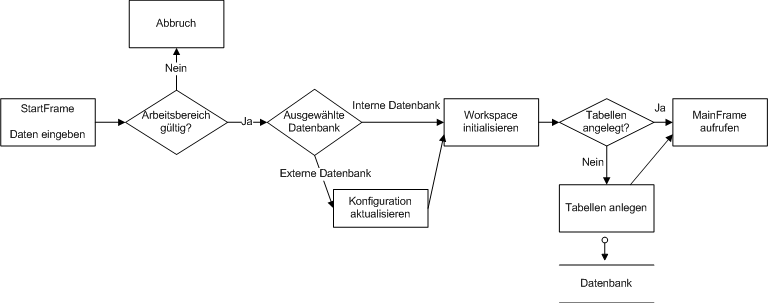
\includegraphics[width=\gfxwidth]{gfx/Ablauf_start}
\caption{/F0001/ Ablaufplan: Programmstart}
\label{img:Ablauf_start}
\end{center}
\end{figure}

\paragraph{/F0002/Erstellen einer Veranstaltung:}
Die Planung der Funktion kann dem Pflichtenheft, Kapitel \ref{subsubsec:/F0002/} (S.\pageref{subsubsec:/F0002/}) entnommen werden. Die Umsetzung ist in der Abbildung \ref{img:Ablauf_ve_hinzu} (S.\pageref{img:Ablauf_ve_hinzu}) dargestellt.

\begin{figure}[hb]
\begin{center}
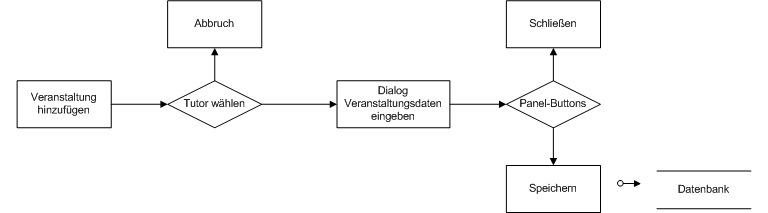
\includegraphics[width=\gfxwidth]{gfx/Ablauf_ve_hinzu}
\caption{/F0002/ Ablaufplan: Eine Veranstaltung hinzuf�gen}
\label{img:Ablauf_ve_hinzu}
\end{center}
\end{figure}

\paragraph{/F0003/Hinzuf�gen von Studenten zu einer Veranstaltung:}
Die Planung der Funktion kann dem Pflichtenheft, Kapitel \ref{subsubsec:/F0003/} (S.\pageref{subsubsec:/F0003/}) entnommen werden. Die Umsetzung ist in der Abbildung \ref{img:Ablauf_studToEvent} (S.\pageref{img:Ablauf_studToEvent}) dargestellt.

\begin{figure}[hb]
\begin{center}
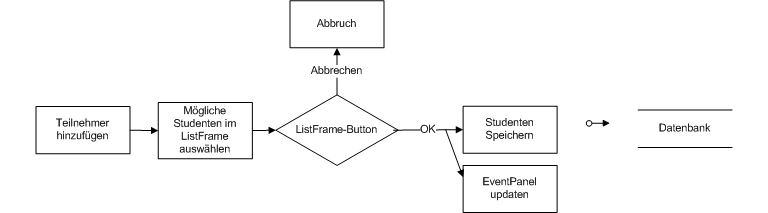
\includegraphics[width=\gfxwidth]{gfx/Ablauf_studToEvent}
\caption{/F0003/ Ablaufplan: Studenten zu einer Veranstaltung hinzuf�gen}
\label{img:Ablauf_studToEvent}
\end{center}
\end{figure}

\paragraph{/F0004/Einteilung der Studenten in Gruppen:} 
Die Planung der Funktion kann dem Pflichtenheft, Kapitel \ref{subsubsec:/F0004/} (S.\pageref{subsubsec:/F0004/}) entnommen werden. Die Umsetzung ist in der Abbildung \ref{img:Ablauf_studToGroup} (S.\pageref{img:Ablauf_studToGroup}) dargestellt.

\begin{figure}[hb]
\begin{center}
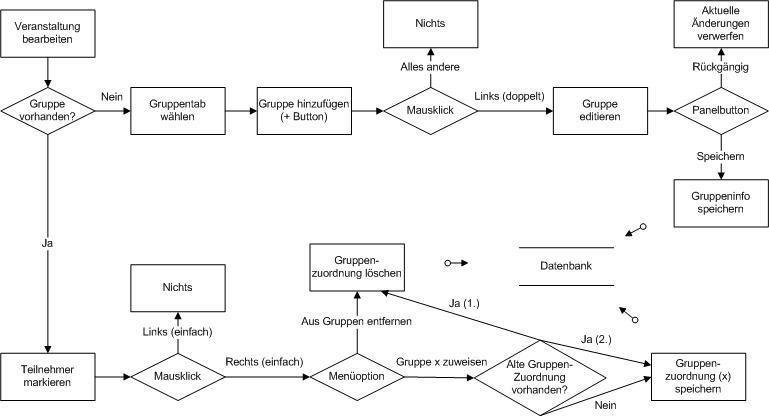
\includegraphics[width=\gfxwidth]{gfx/Ablauf_studToGroup}
\caption{/F0004/ Ablaufplan: Studenten einer Veranstaltung in Gruppen einteilen}
\label{img:Ablauf_studToGroup}
\end{center}
\end{figure}

\paragraph{/F0005/Ein Projekt hinzuf�gen:}
Die Planung der Funktion kann dem Pflichtenheft, Kapitel \ref{subsubsec:/F0005/} (S.\pageref{subsubsec:/F0005/}) entnommen werden. Die Umsetzung ist in der Abbildung \ref{img:Ablauf_addProject} (S.\pageref{img:Ablauf_addProject}) dargestellt.

\begin{figure}[hb]
\begin{center}
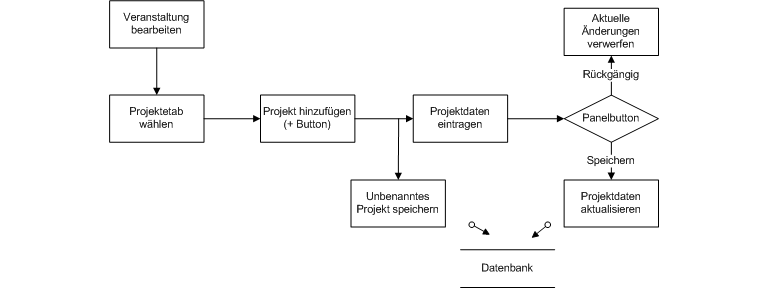
\includegraphics[width=\gfxwidth]{gfx/Ablauf_addProject}
\caption{/F0005/ Ablaufplan: Ein neues Projekt hinzuf�gen}
\label{img:Ablauf_addProject}
\end{center}
\end{figure}

\paragraph{/F0006/Einen Termin hinzuf�gen:}
Die Planung der Funktion kann dem Pflichtenheft, Kapitel \ref{subsubsec:/F0006/} (S.\pageref{subsubsec:/F0006/}) entnommen werden. Die Umsetzung ist in der Abbildung \ref{img:Ablauf_addTerm} (S.\pageref{img:Ablauf_addTerm}) dargestellt.

\begin{figure}[hb]
\begin{center}
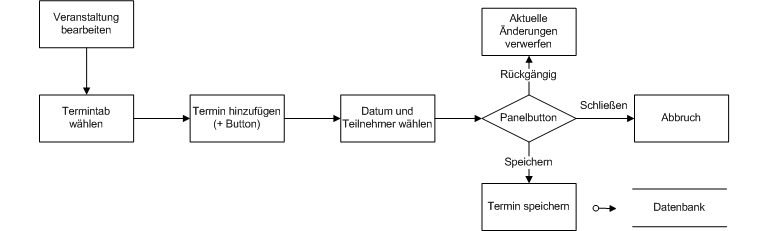
\includegraphics[width=\gfxwidth]{gfx/Ablauf_addTerm}
\caption{/F0006/ Ablaufplan: Einen neuen Termin f�r eine Veranstaltung hinzuf�gen}
\label{img:Ablauf_addTerm}
\end{center}
\end{figure}

\paragraph{/F0007/Den Tutor einer Veranstaltung �ndern:}
Die Planung der Funktion kann dem Pflichtenheft, Kapitel \ref{subsubsec:/F0007/} (S.\pageref{subsubsec:/F0007/}) entnommen werden. Die Umsetzung ist in der Abbildung \ref{img:Ablauf_changeTutor} (S.\pageref{img:Ablauf_changeTutor}) dargestellt.

\begin{figure}[hb]
\begin{center}
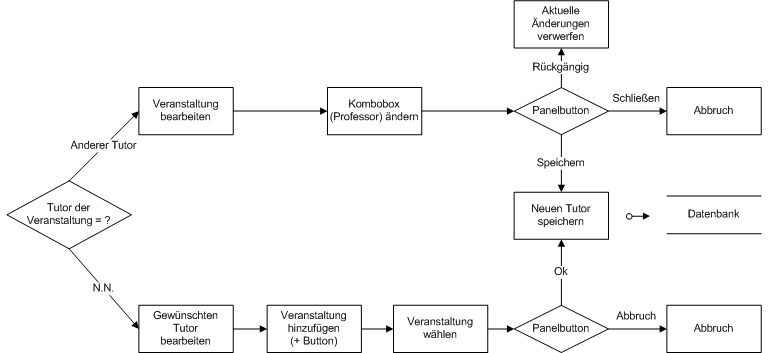
\includegraphics[width=\gfxwidth]{gfx/Ablauf_changeTutor}
\caption{/F0007/ Ablaufplan: Den Tutor einer Veranstaltung �ndern}
\label{img:Ablauf_changeTutor}
\end{center}
\end{figure}

\paragraph{/F0008/Einen neuen Dozenten hinzuf�gen:}
Die Planung der Funktion kann dem Pflichtenheft, Kapitel \ref{subsubsec:/F0008/} (S.\pageref{subsubsec:/F0008/}) entnommen werden. Die Umsetzung ist in der Abbildung \ref{img:Ablauf_tut_hinzu} (S.\pageref{img:Ablauf_tut_hinzu}) dargestellt.

\begin{figure}[hb]
\begin{center}
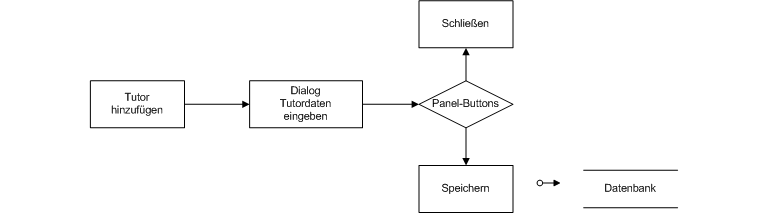
\includegraphics[width=\gfxwidth]{gfx/Ablauf_tut_hinzu}
\caption{/F0008/ Ablaufplan: Einen neuen Dozenten hinzuf�gen}
\label{img:Ablauf_tut_hinzu}
\end{center}
\end{figure}

\paragraph{/F0009/Einen neuen Studenten hinzuf�gen:}
Die Planung der Funktion kann dem Pflichtenheft, Kapitel \ref{subsubsec:/F0009/} (S.\pageref{subsubsec:/F0009/}) entnommen werden. Die Umsetzung ist in der Abbildung \ref{img:Ablauf_stud_hinzu} (S.\pageref{img:Ablauf_stud_hinzu}) dargestellt.

\begin{figure}[hb]
\begin{center}
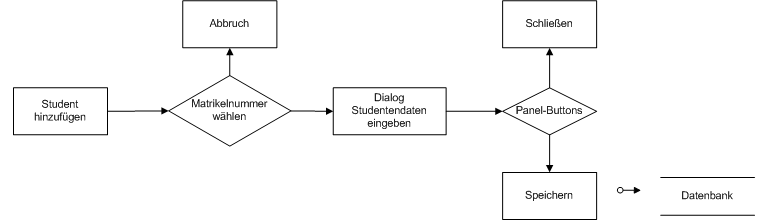
\includegraphics[width=\gfxwidth]{gfx/Ablauf_stud_hinzu}
\caption{/F0009/ Ablaufplan: Einen neuen Studenten hinzuf�gen}
\label{img:Ablauf_stud_hinzu}
\end{center}
\end{figure}

\paragraph{/F0010/Daten in CSV exportieren und /F0011/CSV-Daten importieren:}
Die Planung der Funktion kann dem Pflichtenheft, Kapitel \ref{subsubsec:/F0010/} (S.\pageref{subsubsec:/F0010/}) entnommen werden. Die Umsetzung ist in der Abbildung \ref{img:Ablauf_csv} (S.\pageref{img:Ablauf_csv}) dargestellt.

\begin{figure}[hb]
\begin{center}
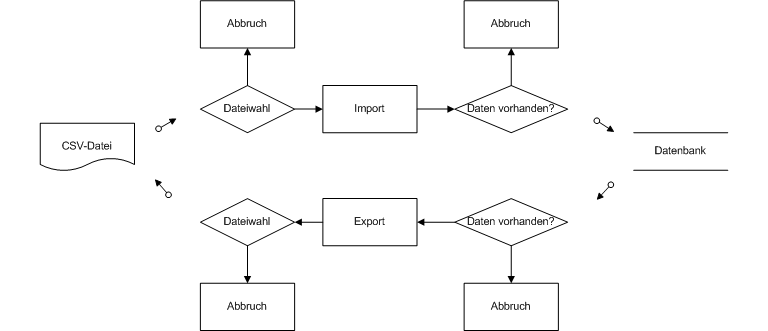
\includegraphics[width=\gfxwidth]{gfx/Ablauf_csv}
\caption{/F0010/ und /F0011/ Ablaufplan: CSV-Import/Export}
\label{img:Ablauf_csv}
\end{center}
\end{figure}

\paragraph{/F0012/Ein Projekt benoten}
Die Planung der Funktion kann dem Pflichtenheft, Kapitel \ref{subsubsec:/F0012/} (S.\pageref{subsubsec:/F0012/}) entnommen werden. Die Umsetzung ist in der Abbildung \ref{img:Ablauf_benoten} (S.\pageref{img:Ablauf_benoten}) dargestellt.

\begin{figure}[hb]
\begin{center}
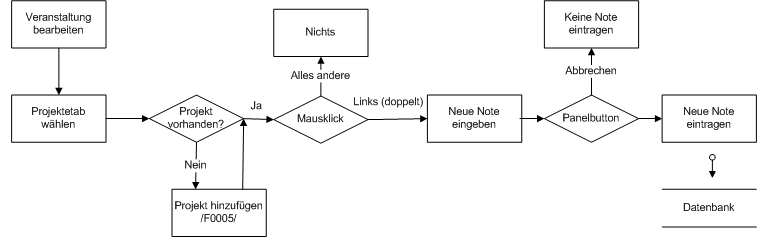
\includegraphics[width=\gfxwidth]{gfx/Ablauf_benoten}
\caption{/F0012/ Ablaufplan: Ein Projekt benoten}
\label{img:Ablauf_benoten}
\end{center}
\end{figure}

% experimentell
\clearpage

\section{Anwendungsgrenzen und Fehlersituationen}
\label{sec:AnwendungsgrenzenFehlersituationen}
``PrakMan'' erlaubt es bei Verwendung einer externen Datenbank, dass mehrere Benutzer auf der selben Datenbasis arbeiten. In diesem Fall k�nnen Probleme auftreten, falls unterschiedliche Benutzer gleichzeitig versuchen, die selben Datens�tze zu ver�ndern. In den meisten F�llen konnte diesem Problem mit dem gezielten Einsatz von Batches entgegengewirkt werden. Alle Problemsituationen k�nnen damit jedoch nicht sicher umgangen werden.
\paragraph{Ein Beispiel: L�schen und Editieren eine Veranstaltung:}
Dozent ``A'' und Dozent ``B'' greifen beide auf die selbe Datenbank ``DB'' zu. A �ffnet nun die Veranstaltung ``VC`` in seinem Programm in einem Tab. Kurz danach l�scht B die Veranstaltung VC aus der Datenbank DB. A m�chte nun, neue Mitglieder zu VC hinzuf�gen und w�hlt diese aus. Sobald A diese Informationen in DB �bertragen hat, ist VC auf einmal wieder vorhanden - jedoch ohne Projekte, Noten und Termine.

Diese F�lle stellen nicht wirklich einen Fehler dar, zeigen jedoch das Problem, das besteht, weil Datenbank und Programm nicht st�ndig auf dem gleichen Stand gehalten werden k�nnen.

\section{Benutzeroberfl�chenhierarchie}
\label{sec:BOFhierarchie}
In ``PrakMan'' existiert ein Hauptfenster, der ``MainFrame''. In diesem befindet sich auf der linken Seite ein Baum, auf der rechten Seite ein ``TabbedPane'', welches unterschiedliche Panels h�lt, die die Informationen der Objekte aus dem Baum f�r den Benutzer darstellen.

Den Zusammenhang bzw. die Hierarchie dieses Bereichs stellt die Abbildung \ref{img:BOF_MainFrame_Panels} (S.\pageref{img:BOF_MainFrame_Panels}) dar.

\begin{figure}[hb]
\begin{center}
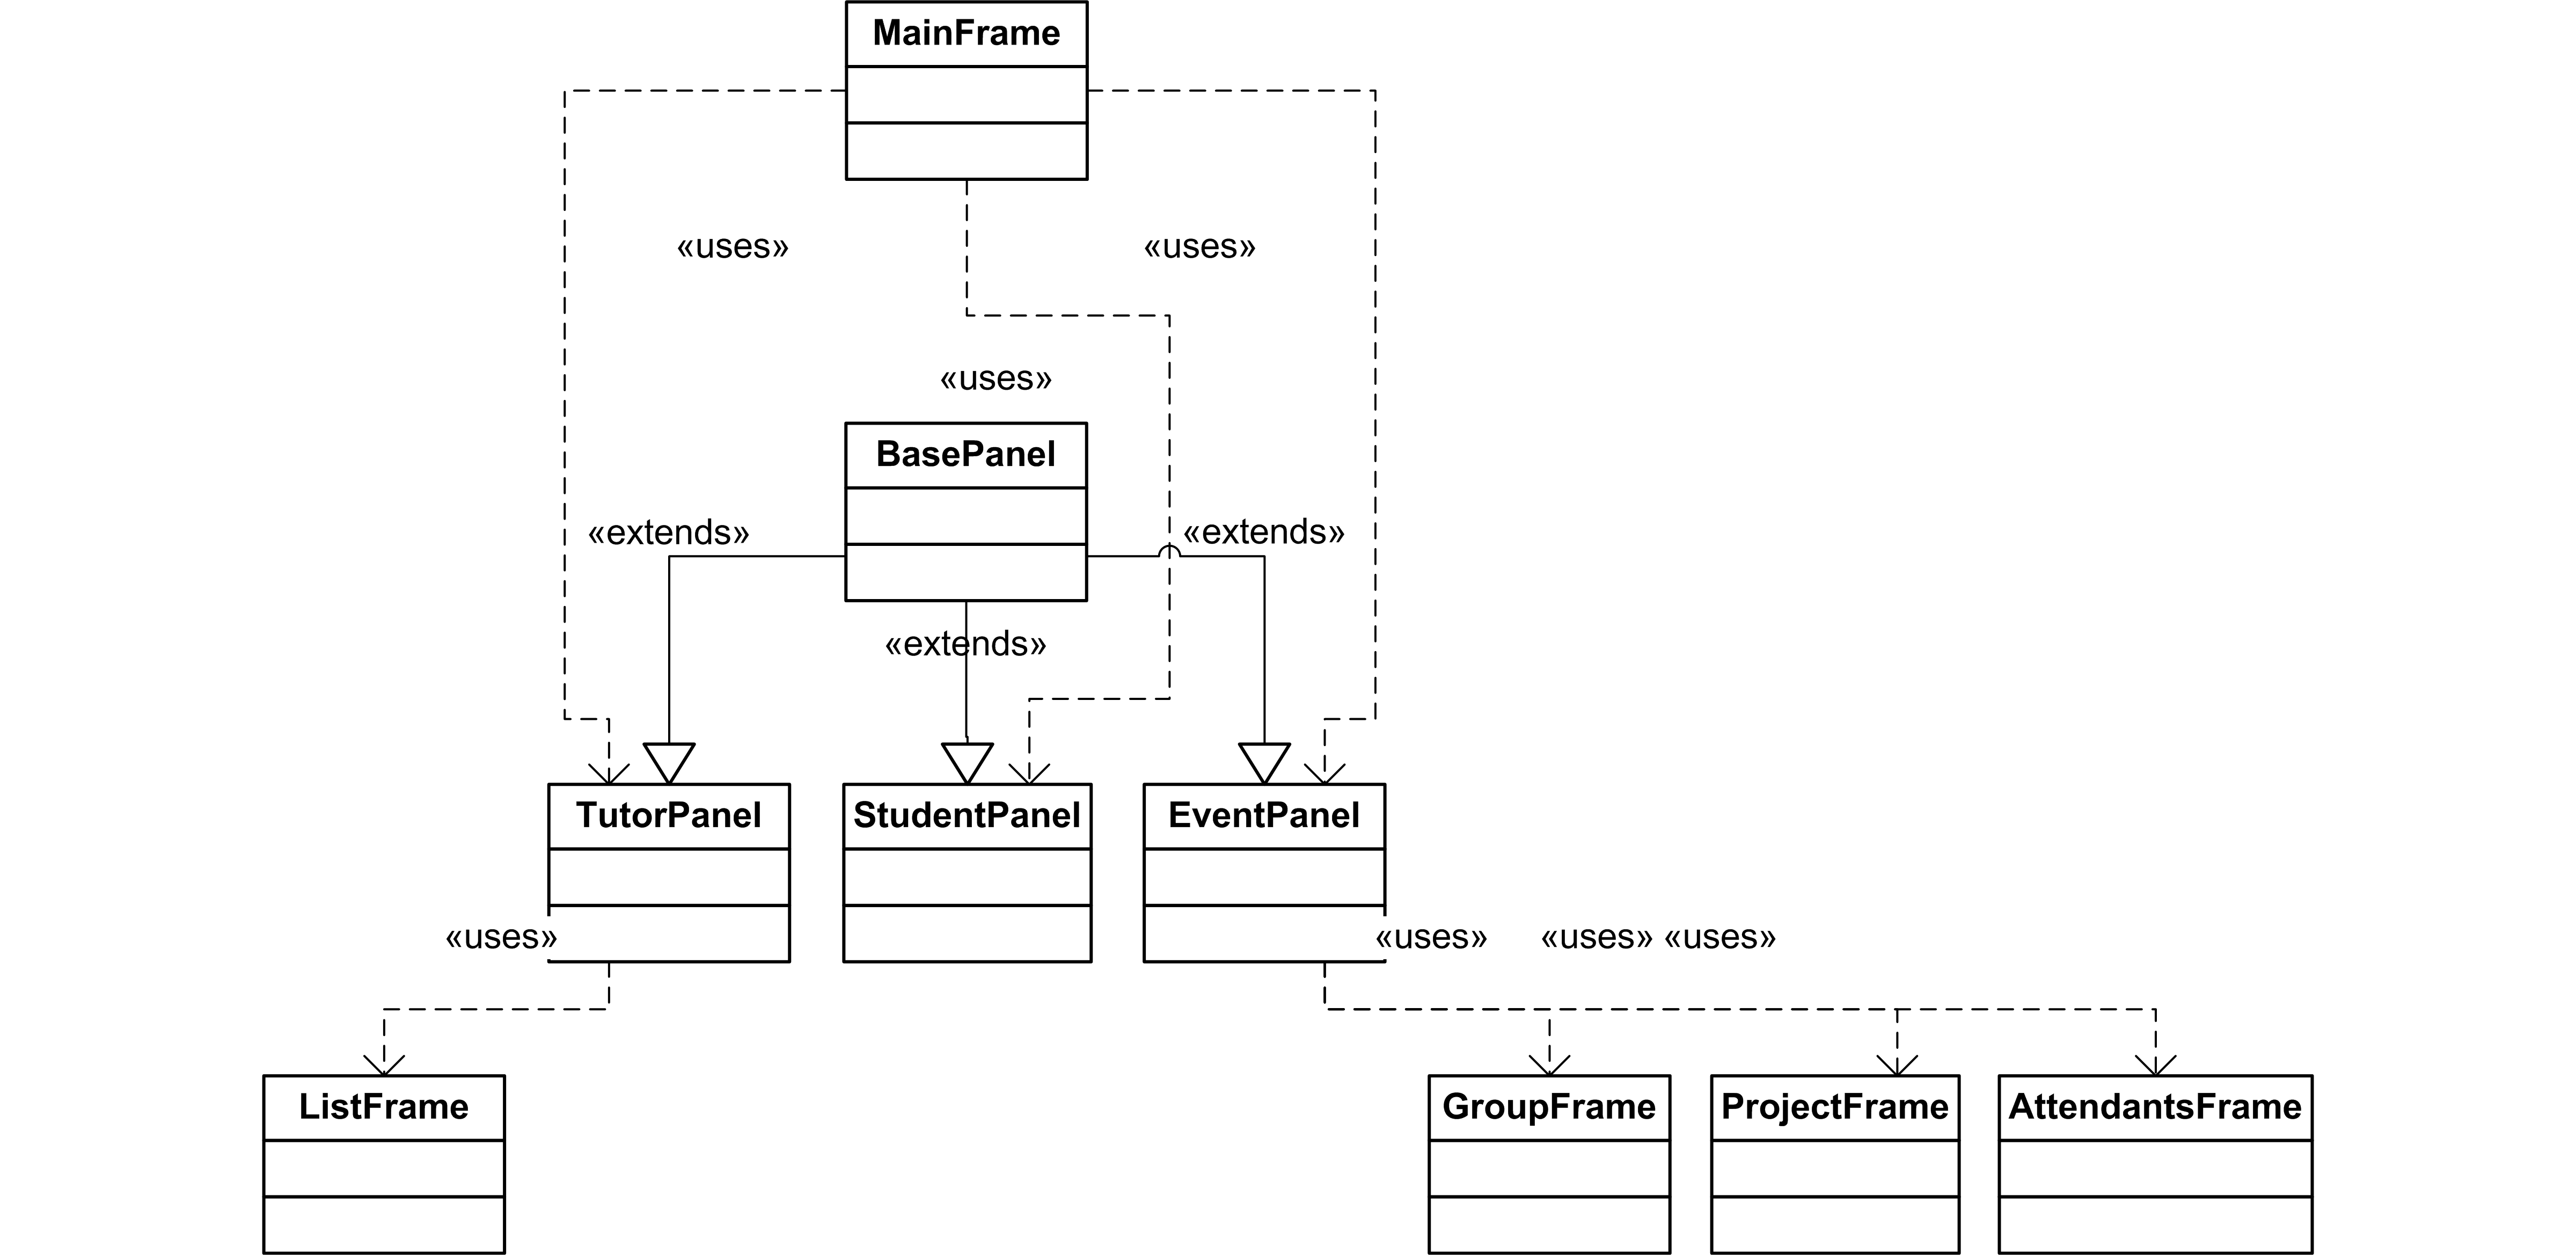
\includegraphics[width=\gfxwidth]{gfx/BOF_MainFrame_Panels}
\caption{Ablaufplan: Hierarchie der Benutzeroberfl�che, ausgehend vom MainFrame}
\label{img:BOF_MainFrame_Panels}
\end{center}
\end{figure}

Abbildung \ref{img:BOF_Workspace_Tree} (S.\pageref{img:BOF_Workspace_Tree}) geht weiter auf den speziellen Aufbau der Kontextmen�s im Baum (linke Seite der Benutzeroberfl�che) ein.

\begin{figure}[hb]
\begin{center}
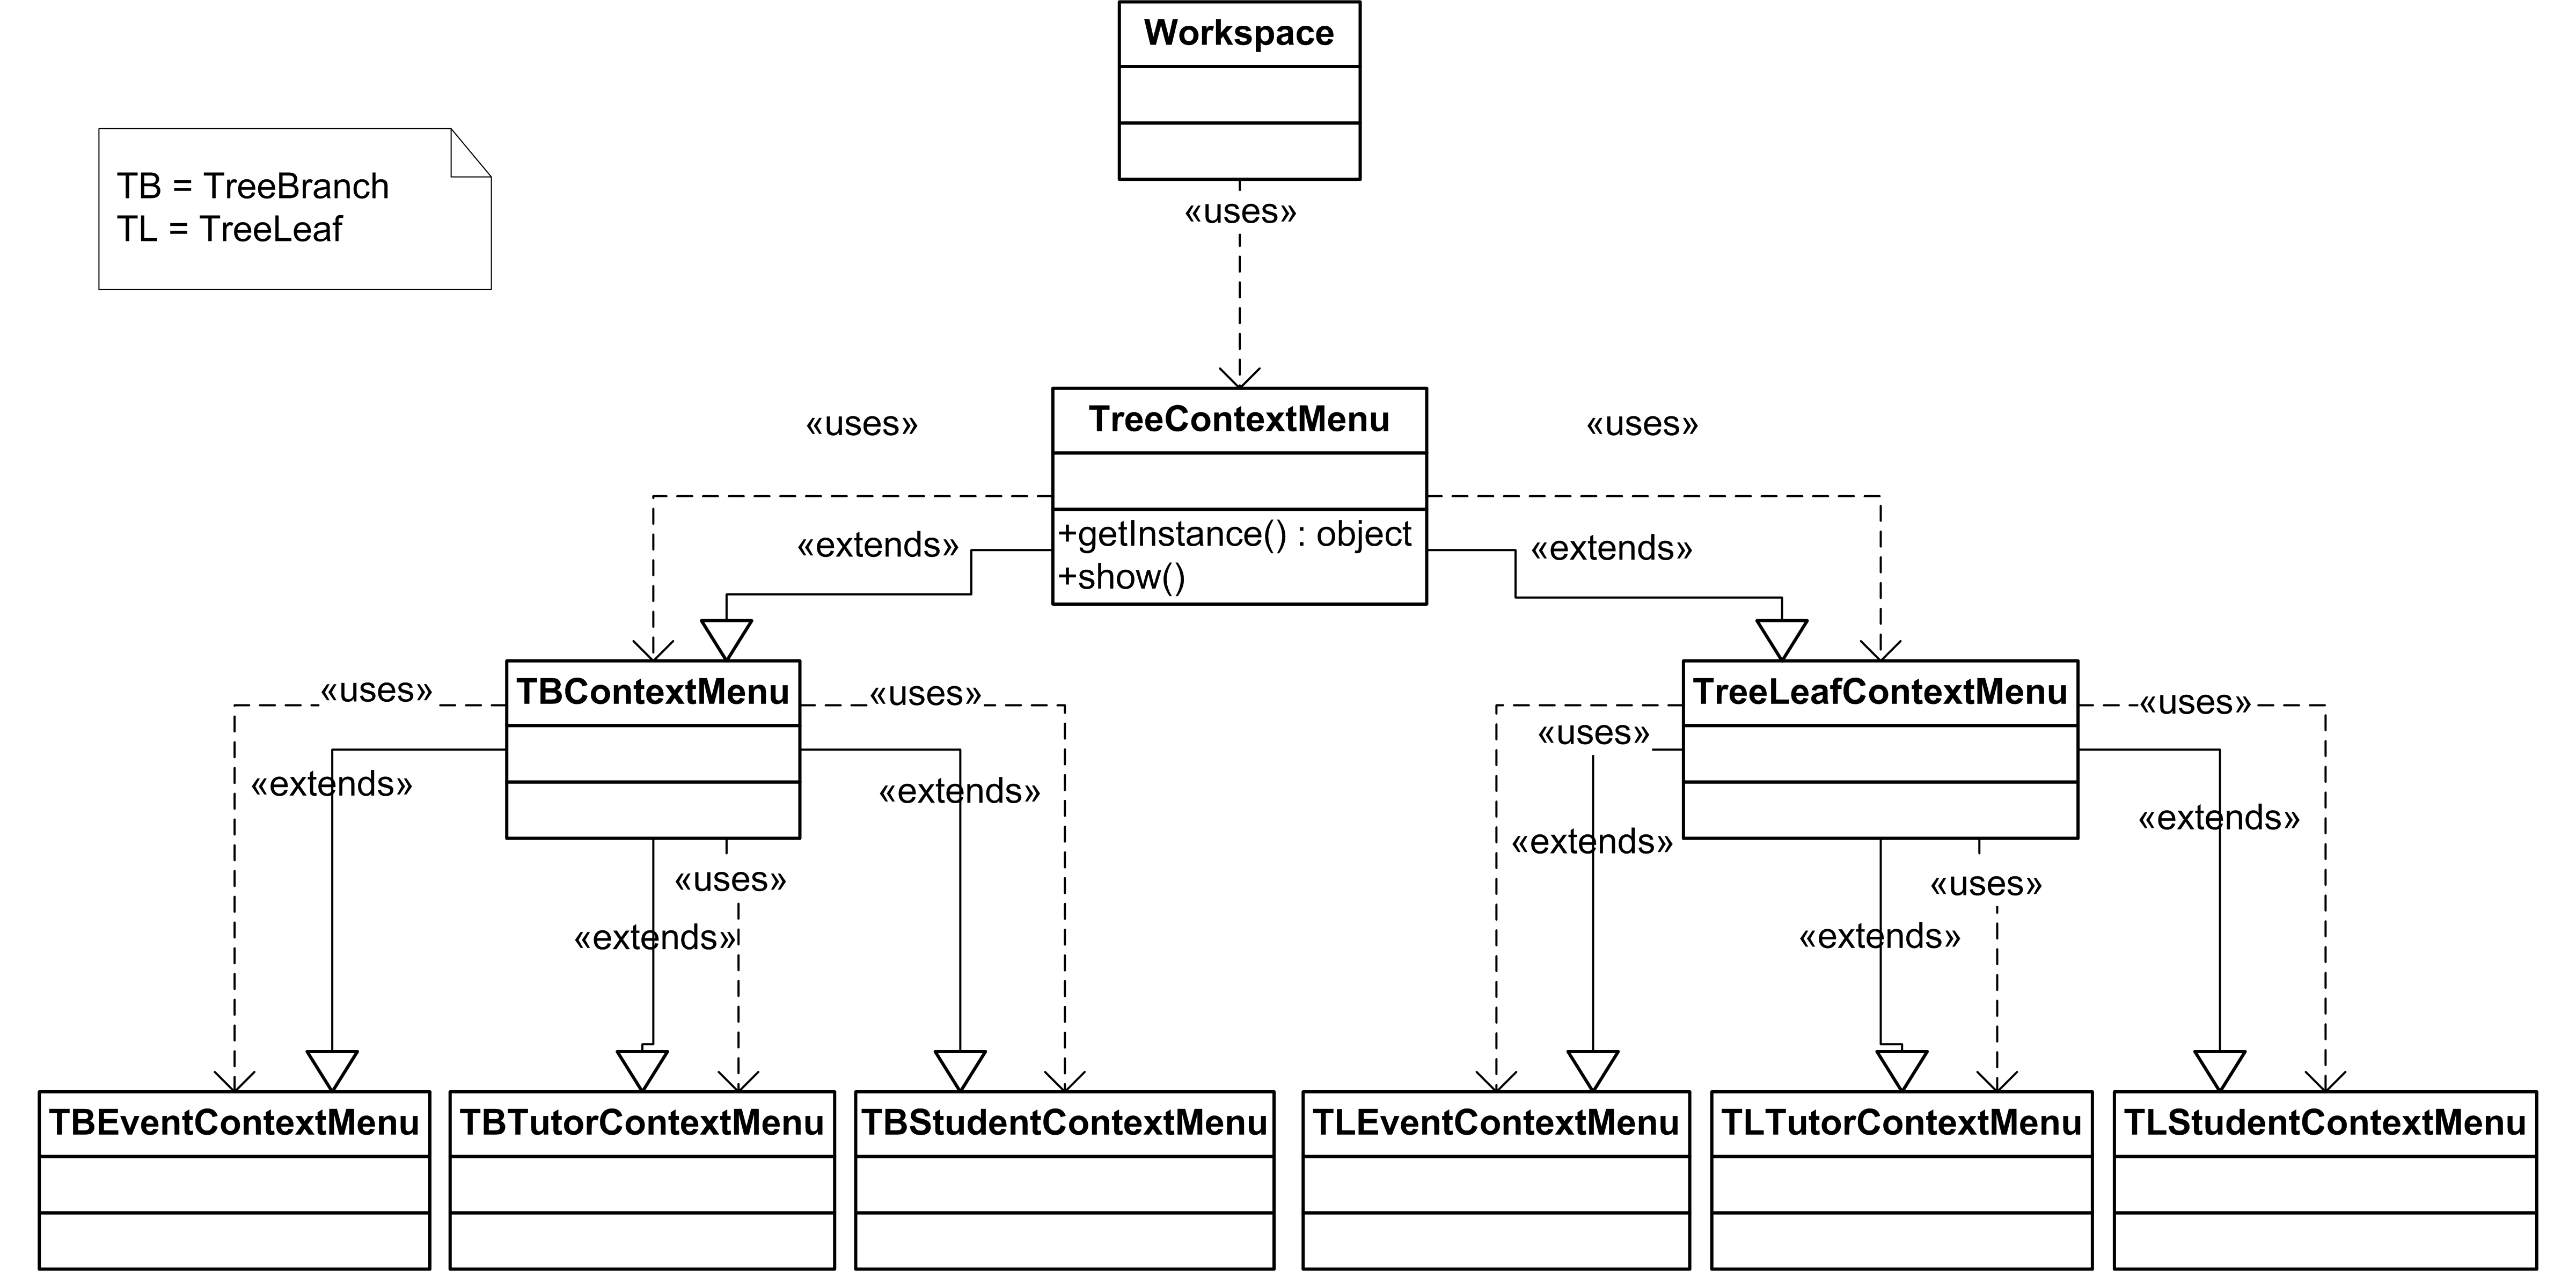
\includegraphics[width=\gfxwidth]{gfx/BOF_Workspace_Tree}
\caption{Ablaufplan: Hierarchie der Benutzeroberfl�che, speziell des Baumes, ausgehend vom Workspace}
\label{img:BOF_Workspace_Tree}
\end{center}
\end{figure}

% experimentell
\clearpage

\section{Funktionsbeschreibung der Benutzeroberfl�chen und deren Komponenten}
\label{sec:BOFBeschreibung}
Exemplarisch die Zusammenstellung der wichtigsten GUI-Masken und eine Beschreibung ihrer Funktion(en):

\paragraph{MainFrame} = JMenuBar + txtFilter + splitPane + Workspace (Tree) + tabbedPane + [ EventPanel | TutorPanel | StudentPanel ]

Im Mainframe laufen alle Fenster zusammen. Er stellt das �u�ere Ger�st dar, zu welchem der Baum geh�rt, der alle O
bjekte �bersichtlich zur Verf�gung stellt, sowie die Men�leiste, welche weitere Optionen anbietet. Au�erdem erlaubt er durch eine ``splitPane'' das einfache Ver�ndern der Gr��e der beiden Teilbereiche des Hauptfensters. Zuletzt ist auch das ``tabbedPane'', in welchem weitere Unterpanels angezeigt werden, ein Teil dieses Hauptfensters.

\paragraph{BasePanel} = JPanel

Das BasePanel stellt eine Basisklasse f�r weitere Objektpanels dar. Es legt  haupts�chlich abstrakte Methoden fest, die in den abgeleiteten Klassen implementiert werden m�ssen. Ansonsten ist es ein einfaches JPanel, das anschlie�end mit Inhalten gef�llt werden kann.

\paragraph{EventPanel} = BasePanel + SaveResetEditPanel + eventContentPanel + tabbedPane + [ eventMemberPanel | eventResultPanel | eventTermsPanel | eventGroupsPanel ]

Das EventPanel ist eine Ableitung des BasePanel und wird im ``tabbedPane'' des MainFrame angezeigt. Dieses Panel zeigt alle Informationen an, die �ber eine Veranstaltung existieren. Dazu geh�ren eine Beschreibung, die Teilnehmer, Arbeitsgruppen, Projekte bzw. Hausarbeiten, und Termine sowie Anwesenheitslisten f�r Letztere. All diese Daten k�nnen �ber das Panel auch editiert werden. Es erlaubt somit eine umfassende Administration einer gew�hlten Veranstaltung.

\paragraph{TutorPanel} = BasePanel + SaveResetEditPanel + tutorContentPanel +  tabbedPane + [ tutorPraktPanel ]

Das TutorPanel stellt ebenfalls eine Ableitung des BasePanel dar und wird an der gleichen Stelle angezeigt. Hier k�nnen Dozenten-bezogene Daten gefunden werden: Vorname, Nachname und welche Veranstaltungen vom gew�hlten Dozenten angeboten werden. All diese Informationen lassen sich wiederum editieren.

\paragraph{StudentPanel} = BasePanel + SaveResetEditPanel + studentContentPanel +  tabbedPane + [ studentPraktPanel |  studentResultsPanel ]

Auch das StudentPanel ist eine Ableitung des BasePanel und wird im ``tabbedPane'' des MainFrame angezeigt. Hier k�nnen Studenten-bezogene Daten eingesehen und editiert werden: Vorname, Nachname, E-Mail-Adresse, an welchen Veranstaltungen nimmt der/die Student/in teil und welche Projekte werden bearbeitet oder wurden auch schon benotet. Die beiden letztgenannten Funktionen m�ssen allerdings �ber eine Veranstaltung vorgenommen werden und k�nnen hier lediglich angezeigt werden. Die Tabellen bieten daf�r allerdings die M�glichkeit, �ber einen Doppelklick auf Veranstaltungs/Tutor/Studenten -daten das entsprechende Objekt separat zu �ffnen, um dort direkt weiterarbeiten zu k�nnen.


\section{Dateiaufbau aller Anwenderdateien mit DD- Beschreibung und Funktion}
\label{sec:DateiaufbauAnwenderdateien}
% Formatierung der CSV-Daten
\subsection{Export von Studentendaten:}
\label{subsec:Dateiaufbau_CSV_Studenten}
Beim Exportieren von Studentendaten werden Vorname, Nachname, Matrikelnummer und E-Mail-Adresse in einer CSV-Datei gespeichert. Der Aufbau sieht folgenderma�en aus.

\paragraph{studenten.csv} = Vorname + Name + E-Mail + Matrikelnummer

\subsection{Export von Dozentendaten:}
\label{subsec:Dateiaufbau_CSV_Dozenten}
Beim Exportieren von Dozentendaten werden Vorname, Nachname sowie eine intern vergebene Dozenten-ID in einer CSV-Datei gespeichert. Der Aufbau sieht folgenderma�en aus.

\paragraph{dozenten.csv} = Vorname + Name + Tutor-ID

\subsection{Export von Veranstaltungsdaten:}
\label{subsec:Dateiaufbau_CSV_Veranstaltung}
Beim Exportieren von Daten einer gew�hlten Veranstaltung werden alle verf�gbaren Informationen in einer mehrschichtigen CSV-Datei zusammengestellt. Alle Zeitangaben werden als Unix-Timestamp exportiert. Der Aufbau dieser CSV ist etwas komplexer und sieht folgenderma�en aus.

\paragraph{veranstaltung.csv} = Veranstaltungs-Info + Tutor-Info + Studenten-Info + Projekt-Info + Benotungs-Info + Termin-Info

Alle Informations-Abschnitte sind durch eine Leerzeile sowie eine Zeile, in der die Bezeichnung der Spalten untergebracht ist, getrennt.

\paragraph{Veranstaltungs-Info} = Veranstaltungsname + Veranstaltungs-ID

\paragraph{Tutor-Info} = Tutor-ID + Nachname + Vorname

\paragraph{Studenten-Info} = Matrikelnummer + Name + Vorname + E-Mail

\paragraph{Projekt-Info} = Projekt-ID + Beschreibung + Startzeit + Endzeit

\paragraph{Benotungs-Info} = Projekt-ID + Matrikelnummer + Note

\paragraph{Termin-Info} = Termin-ID + Zeitpunkt

\chapter{Datenbank}
\label{cha:Datenbank}


\section{Dokumentation der Datenbank}
\label{sec:DokuDerDatenbank}
Als Datenbank ist f�r ``PrakMan'' die Nutzung unterschiedlicher Angebote m�glich. Unterst�tzt werden derzeit Hypersonic-DB (HSQL, sowohl lokal als auch extern) und PostgreSQL. Daf�r wurde der Aufbau der Tabellen relativ einfach gehalten, um allen Datenbanken gerecht zu werden.\\
In den folgenden Abschnitten wird der genaue Aufbau der f�r ``PrakMan'' ben�tigten Tabellen beschrieben bzw. dargestellt.

\section{Entity- Relationship- Modell (ERM) der Datenbank}
\label{sec:ERM}
Der Aufbau der Datenbank, welche f�r den Praktikums-Manager unabdingbar ist, ist in den Grafiken auf den Seiten \pageref{img:ERM-Tutor-Events}, \pageref{img:ERM-Tutor-Events-Projekt} und \pageref{img:ERM-Tutor-Events-Termine} dargestellt. Einige Tabellen werden dabei mehrfach gezeigt, um jeweils den Zusammenhang zu den Grundobjekten (Student, Tutor, Event) darzustellen.

\begin{figure}[hb]
\begin{center}
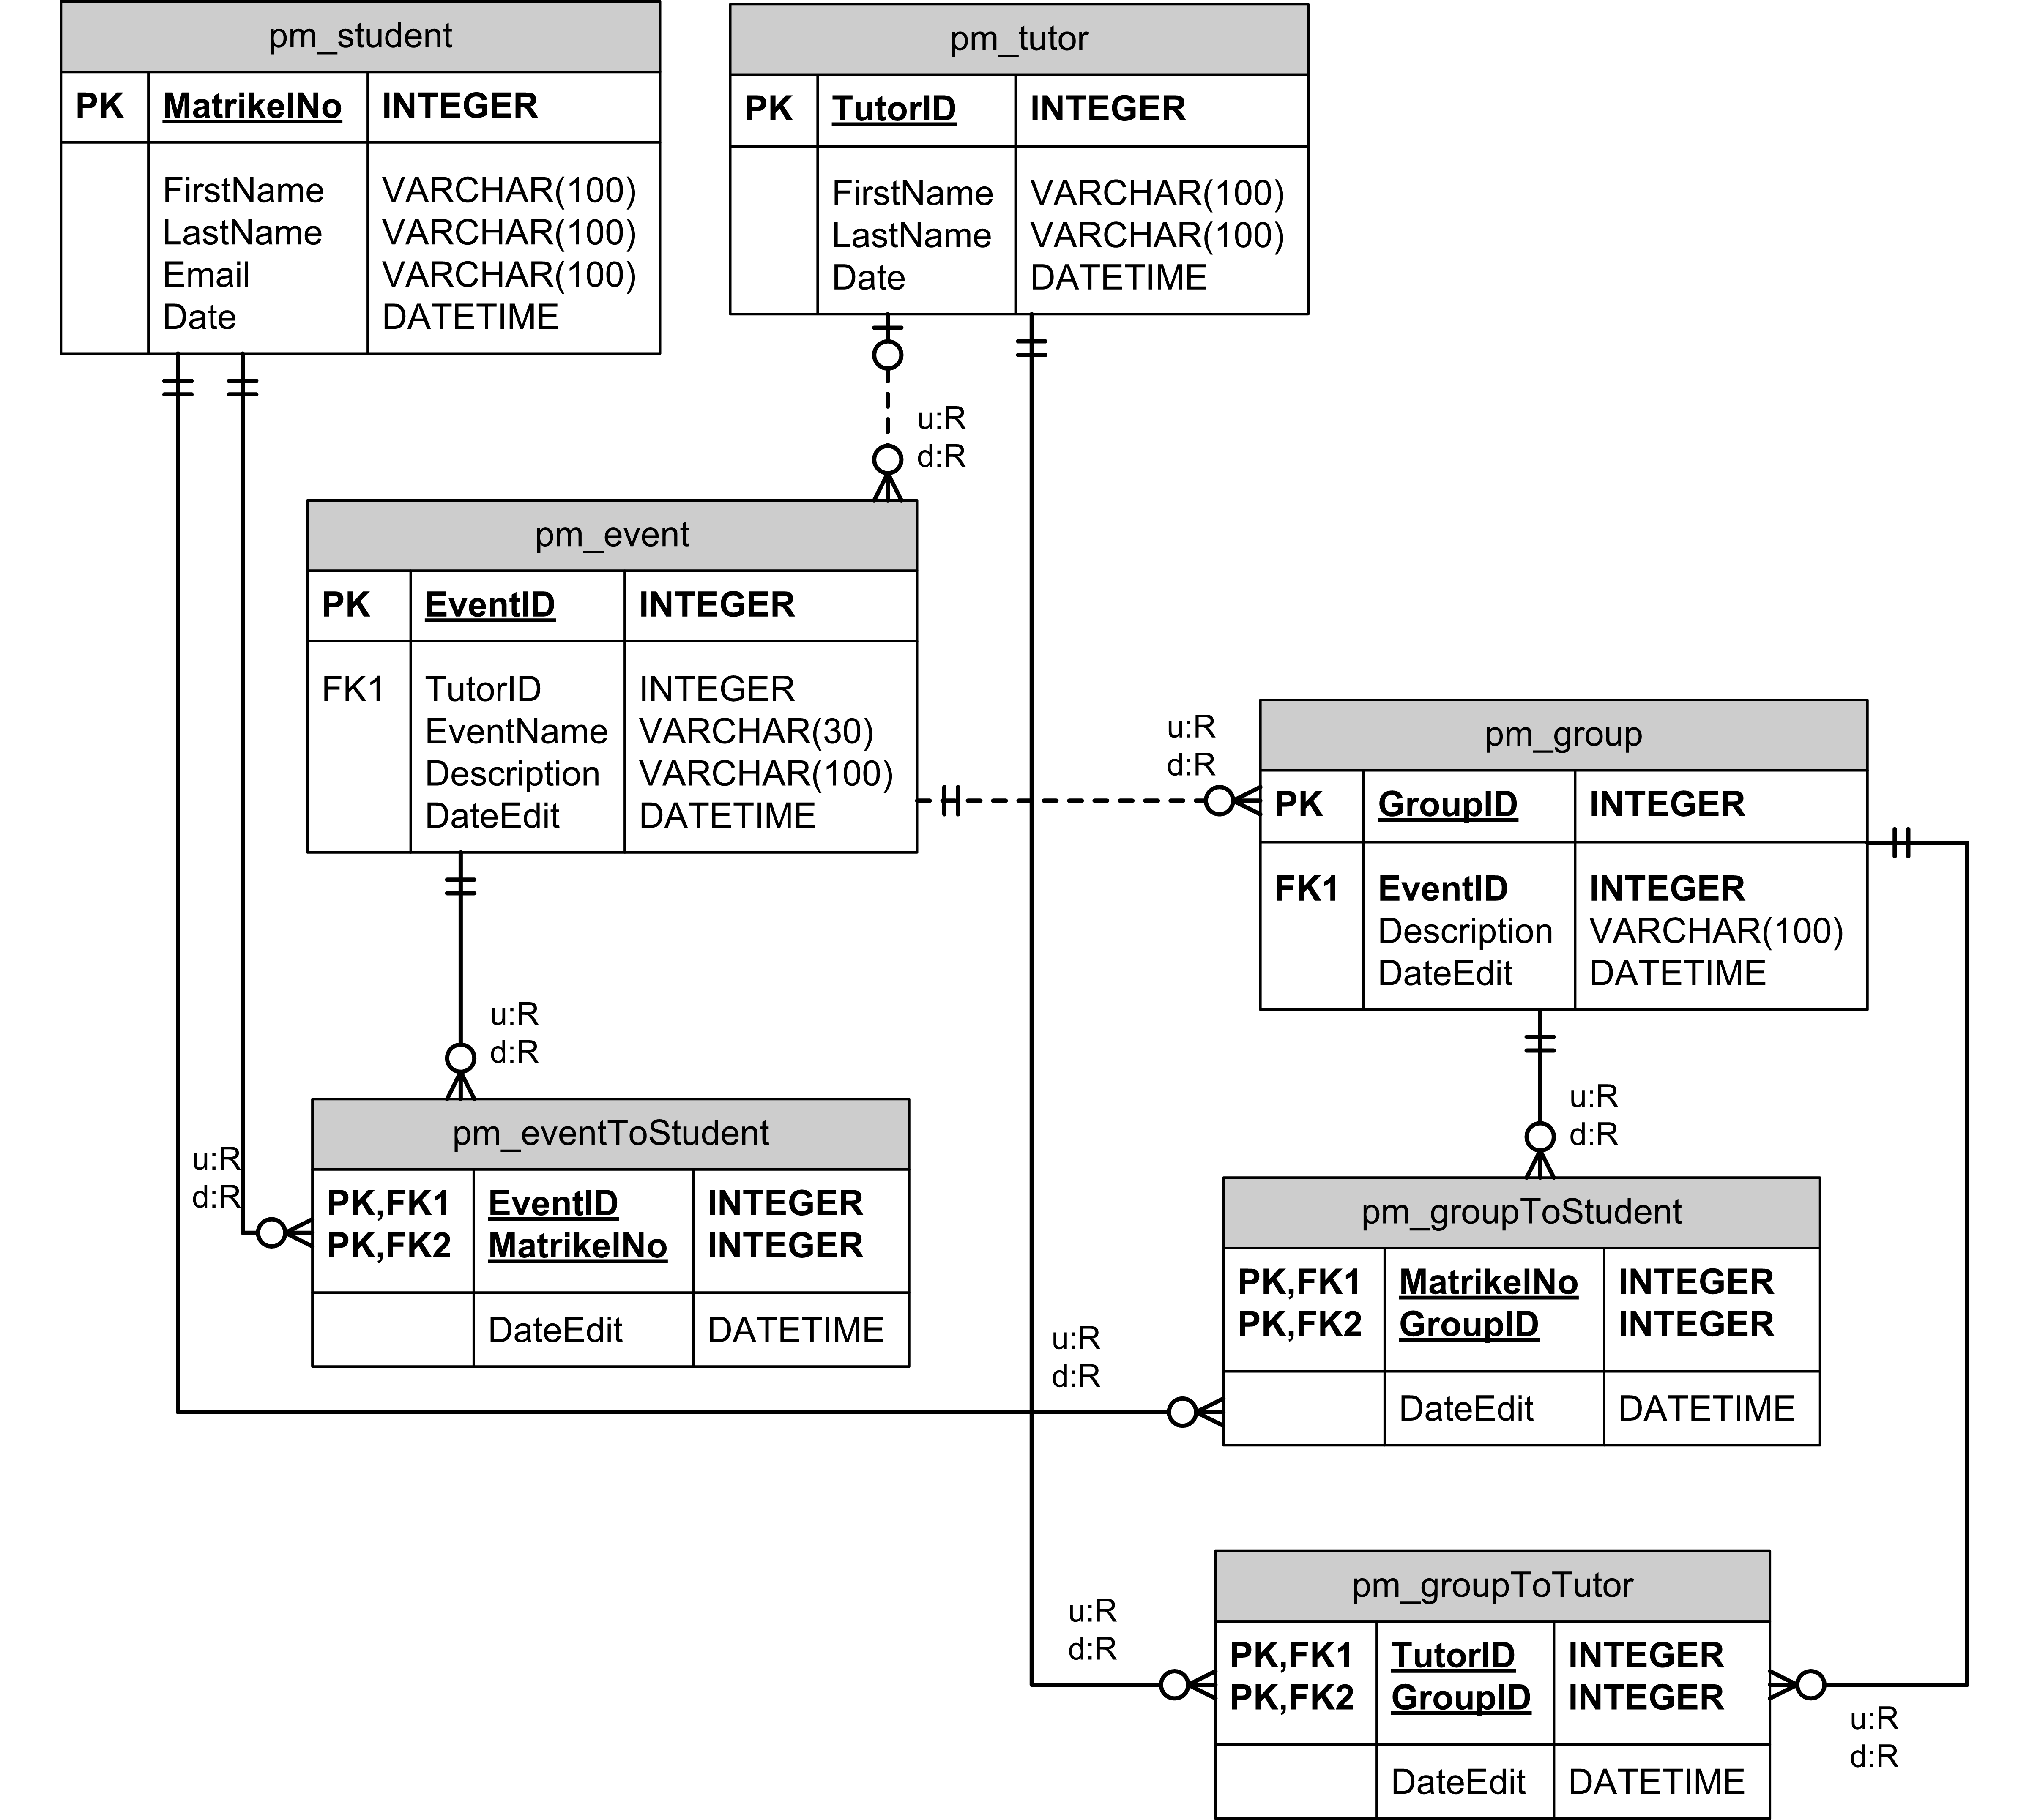
\includegraphics[width=\gfxwidth]{gfx/PrakMan_DB_student_tutor_event}
\caption{ER-Modell der Beziehungen zwischen Student, Tutor und Event}
\label{img:ERM-Tutor-Events}
\end{center}
\end{figure}

\begin{figure}[hb]
\begin{center}
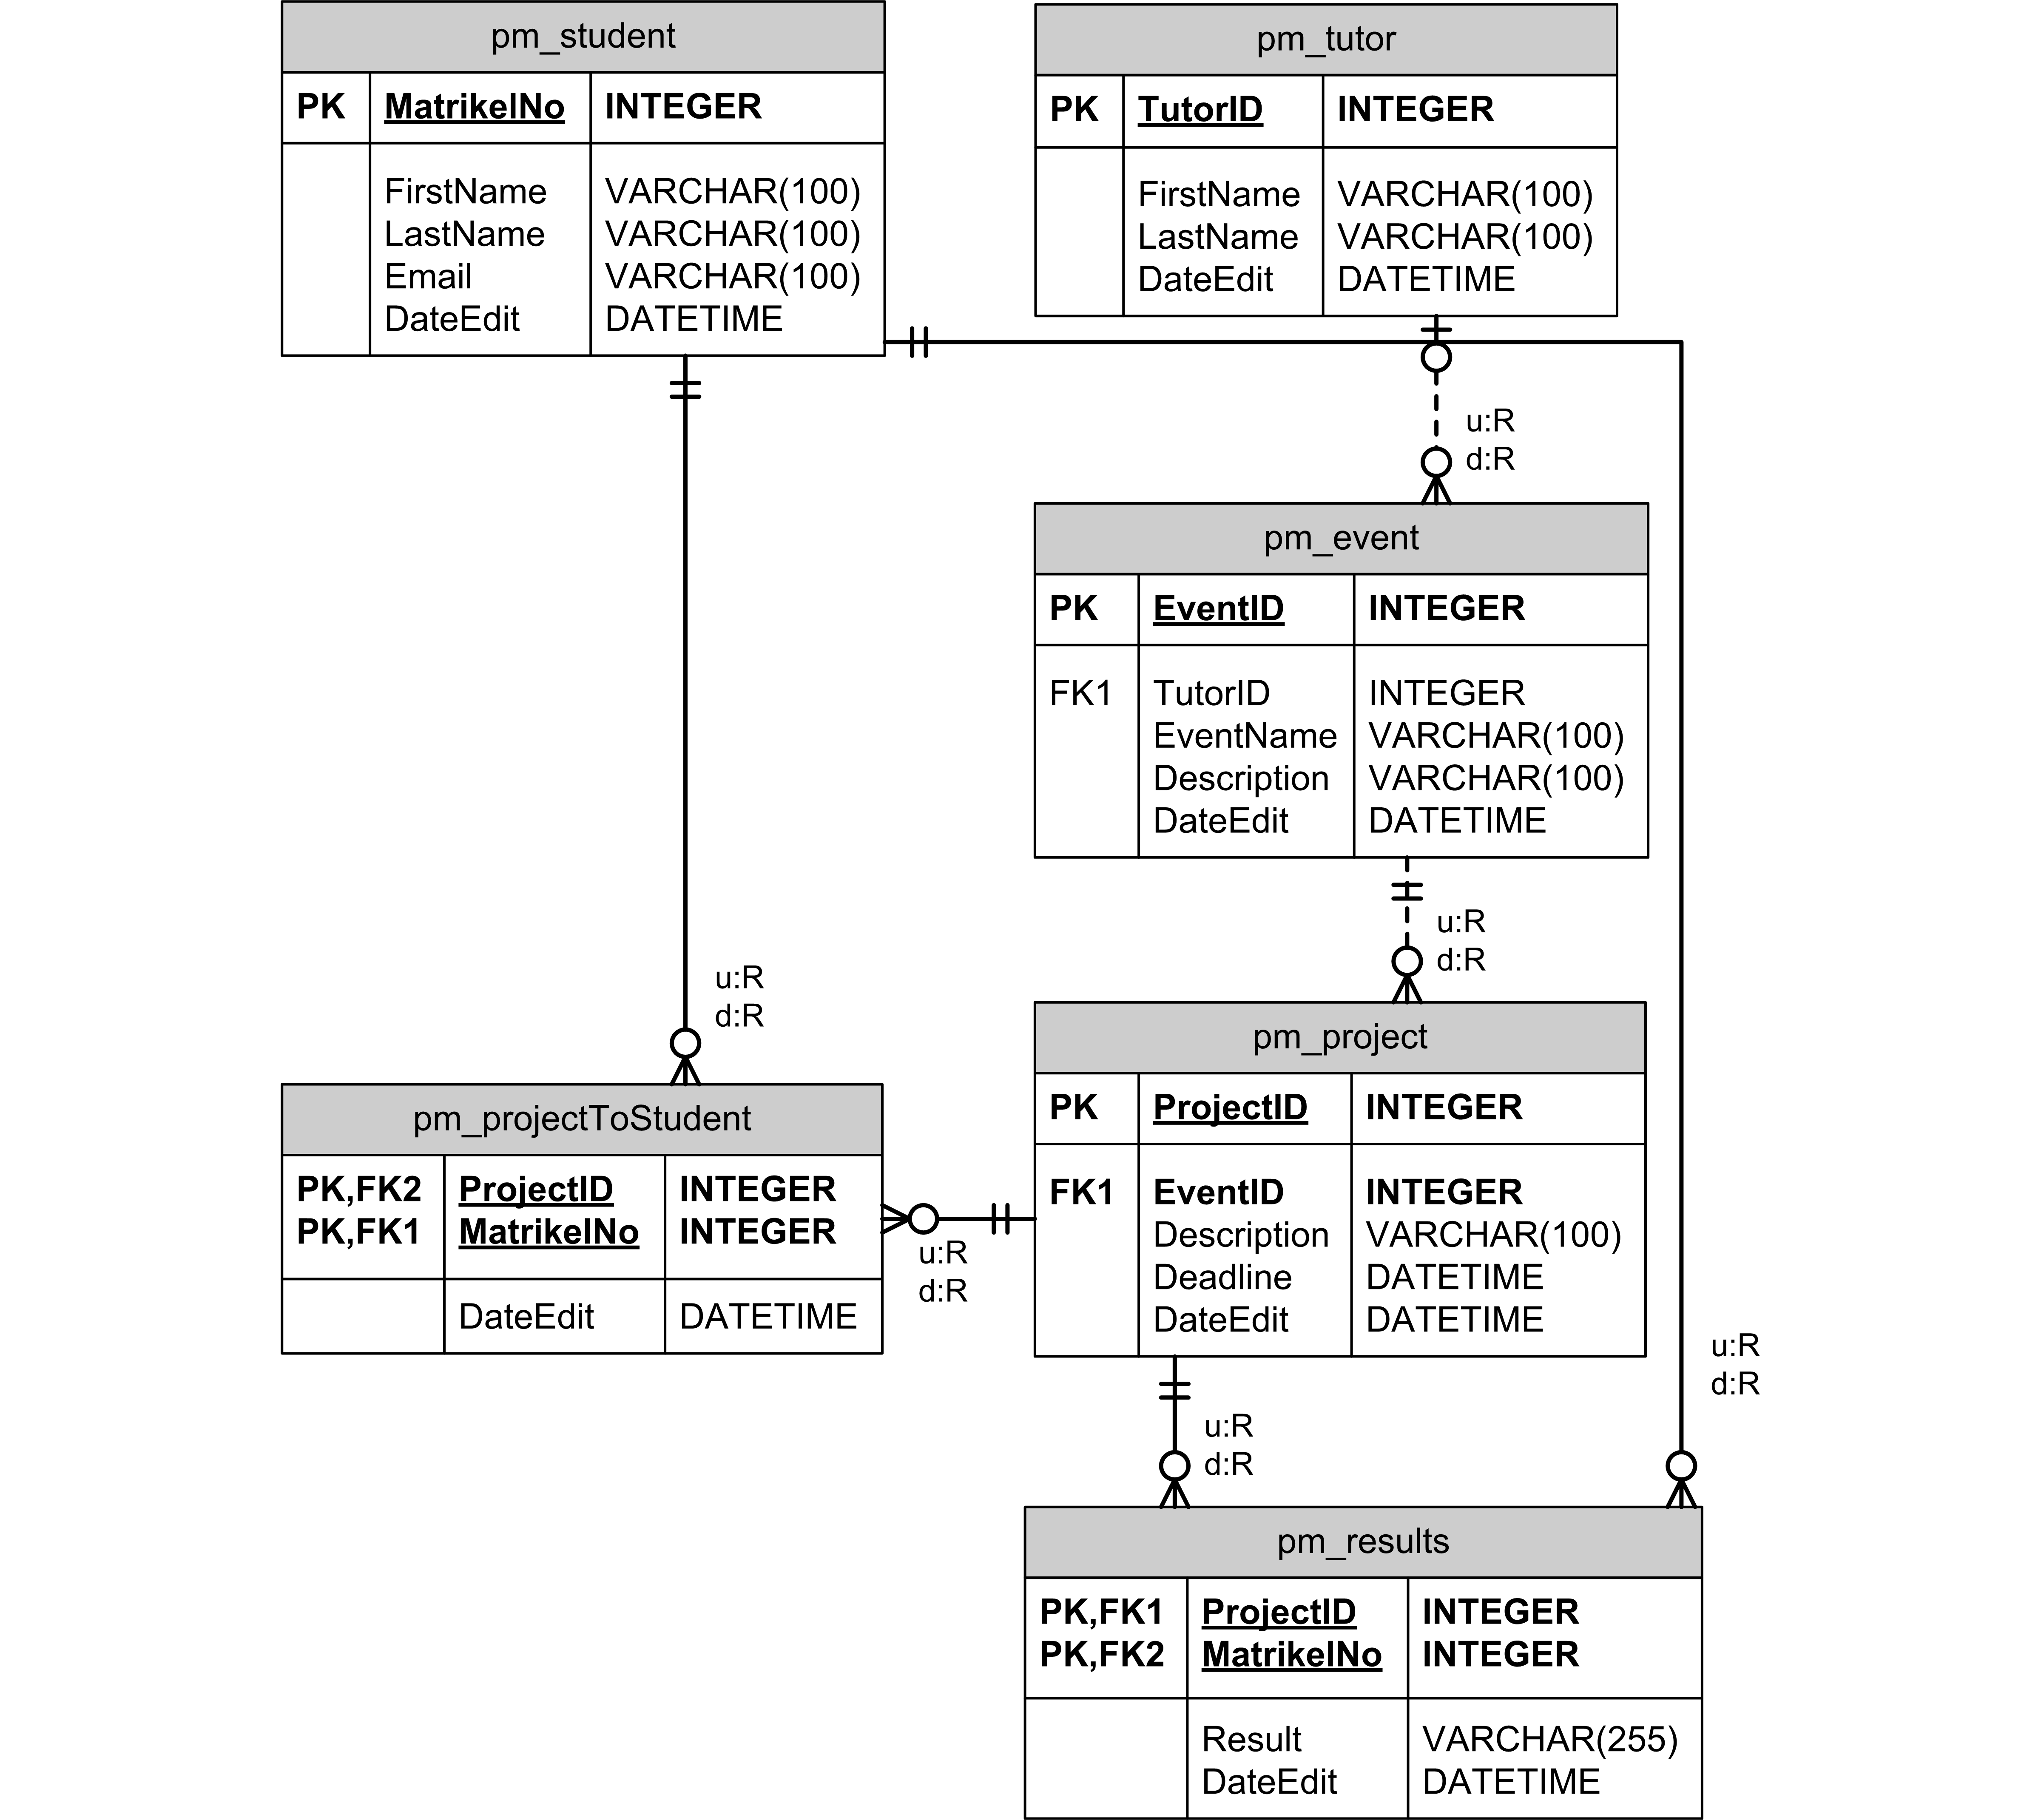
\includegraphics[width=\gfxwidth]{gfx/PrakMan_DB_ERM_event_project}
\caption{ER-Modell der Beziehungen zwischen Student, Tutor, Events und Projekten}
\label{img:ERM-Tutor-Events-Projekt}
\end{center}
\end{figure}

\begin{figure}[hb]
\begin{center}
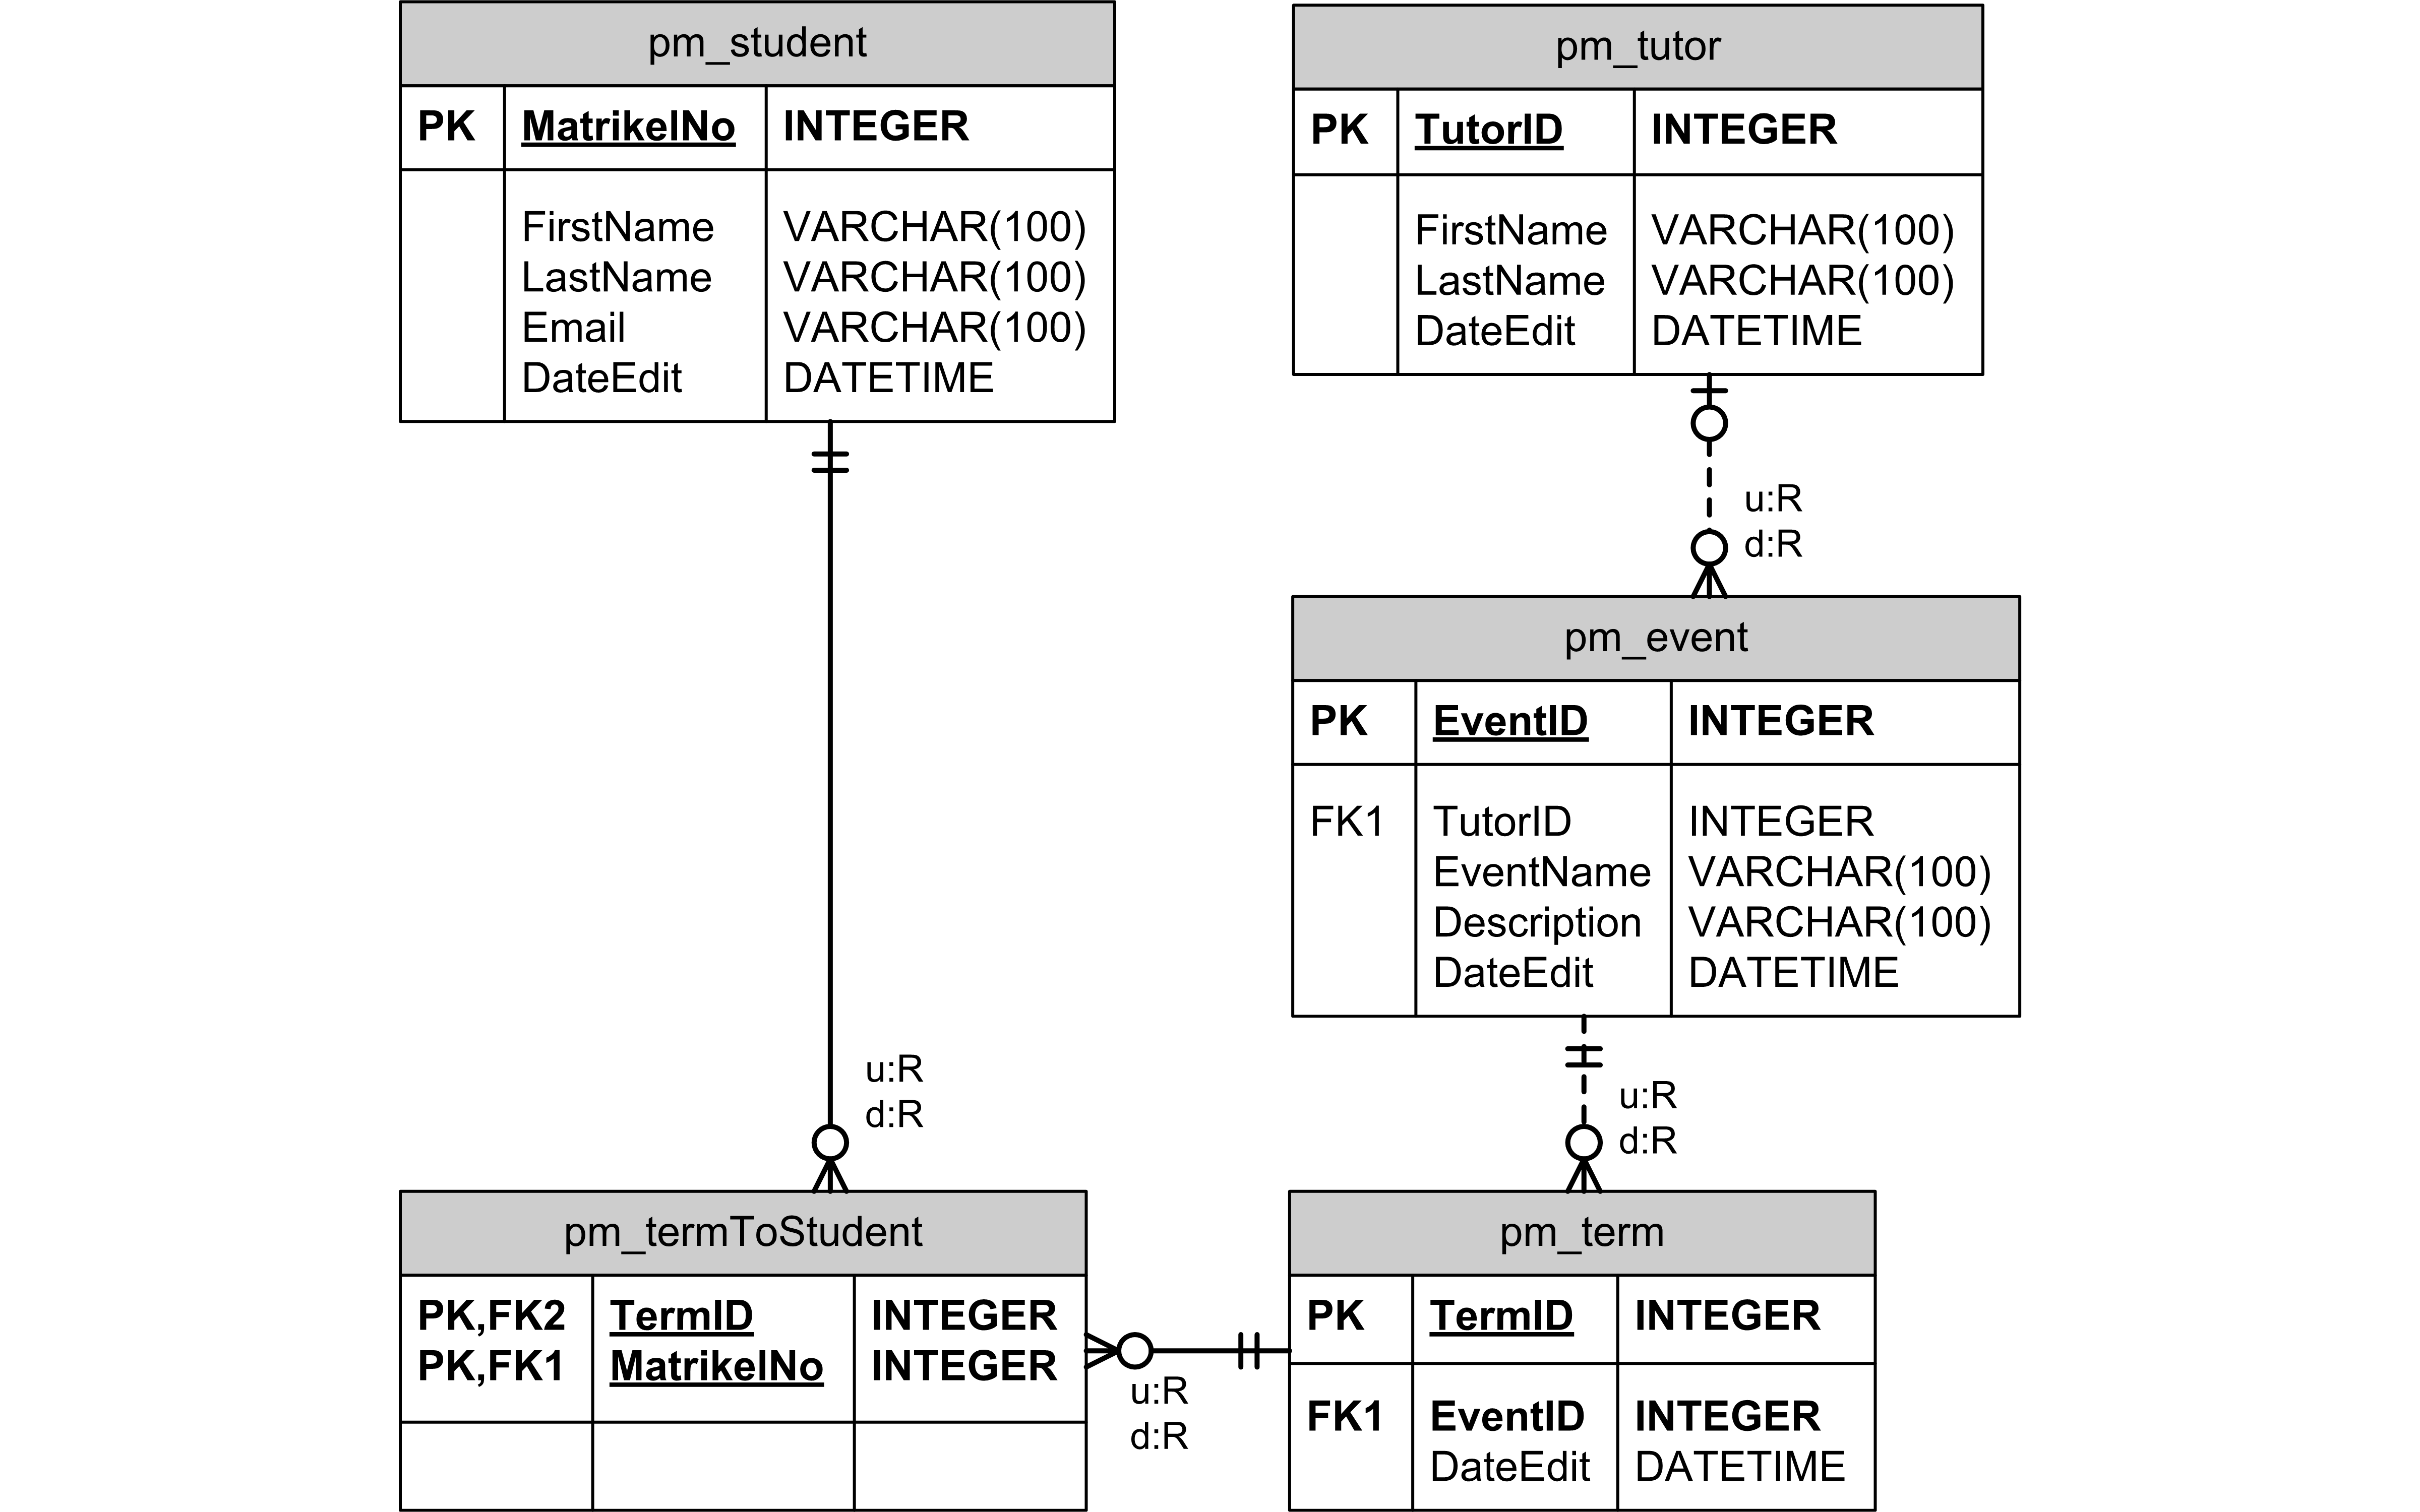
\includegraphics[width=\gfxwidth]{gfx/PrakMan_DB_ERM_terms}
\caption{ER-Modell der Beziehungen zwischen Student, Tutor, Events und Terminen}
\label{img:ERM-Tutor-Events-Termine}
\end{center}
\end{figure}

\section{Pr�fung des Relationenschemas auf Einhaltung der Normalisierung}
\label{sec:PruefungRelationsschema}

\subsection{1te Normalform}
\label{subsec:1teNormalform}
Alle Tabellen enthalten atomare Attribute. Listen werden durch zus�tzliche Tabellen dargestellt.\\
Somit ist 1NF erf�llt.

\subsection{2te Normalform}
\label{subsec:2teNormalform}
Alle Relationen sind in 1NF.
Au�erdem haben alle Objekte (Studenten, Tutoren, Events, Termine, Gruppen, Projekte) eine in der entsprechenden Relation einmalige Identifikationsnummer (ID). Jegliche Verweise laufen ausschlie�lich �ber solche IDs. Somit bestehen auch s�mtliche Prim�rschl�ssel aus einer ID oder mehreren IDs, von denen alle weiteren Attribute voll funktional abh�ngen. Weitere Daten werden f�r Referenzen nicht ben�tigt, weshalb auch keine redundaten Daten in diesem Zusammenhang auftreten k�nnen.\\
Somit ist 2NF erf�llt.

\subsection{3te Normalform}
\label{subsec:3teNormalform}
Alle Relationen sind in 2NF.
Auch hier ist die Eindeutigkeit ausschlie�lich �ber die vorhandenen IDs hergestellt. Keine andere Kombination von Schl�sselkandidaten existiert und w�rde eine weitere Identifikation eines Objekts in einer Tabelle erm�glichen.
Demnach k�nnen auch keine Nicht-Schl�ssel-Attribute von anderen Nicht-Schl�ssel-Attributen funktional abh�ngen.\\
Somit ist 3NF erf�llt.

\section{Funktionsbeschreibung der Formatprogramme}
\label{sec:FunktionsbeschreibungFormatprogramme}

Zum Erstellen der Tabellen wird kein Formatprogramm ben�tigt. Bei Programmstart wird automatisch eine passende SQL-Datei gelesen und die Tabellen, falls n�tig, erstellt.

\section{Funktionsbeschreibung der Reportprogramme}
\label{sec:FunktionsbeschreibungReportprogramme}

Es wurde kein spezielles Reportprogramm zum Auslesen der Datenbank geschrieben, da das, in verbesserter Darstellung, eine Funktion das Programms ``PrakMan'' ist.

\section{Funktionsbeschreibung der SQL- /ESQL- /JDBC- Programme}
\label{sec:FunktionsbeschreibungSQLJDBC}

Wie bereits in Punkt \ref{sec:FunktionsbeschreibungFormatprogramme} erw�hnt, liest ``PrakMan'' zum Erstellen der Tabellen eine SQL-Datei ein und erstellt nach diesen Vorgaben, falls n�tig, das Grundger�st f�r eine korrekte Funktionsweise. Die genannte Datei ist ``CreateTables.sql'', welche sich im Paket prakman.io.sql befindet. Auf diese Weise lassen sich bei �nderung eines Datenbankprogramms auf eine andere Version sehr einfach die Tabellen anpassen.\\
F�r die Zukunft w�re auch eine Erweiterung denkbar, die f�r jede Datenbankform eine extra angepasste SQL-Datei enth�lt, um optimal die M�glichkeiten der unterschiedlichen Datenbanktypen nutzen zu k�nnen.

\chapter{Installation und Test}
\label{chap:InstallationUndTest}

\section{Testverfahren und Testdokumente mit automatischen Tests}
\label{sec:Testverfahren}
Die Software wurde auf unterschiedliche Arten auf korrekte Funktionsweise �berpr�ft. Zuerst individuell durch den Entwickler, der seine Komponente direkt nach Fertigstellung pr�ft. Anschlie�end durch die anderen Entwickler, die diese Komponente im Zusammenspiel mit ihren eigenen testen. Schlie�lich ein Performance-Test durch eine vorher programmierte Automatik. 

\subsection{Individuelle Komponenten-Tests}
\label{subsec:IndividuelleKomponenten-Tests}
Jeder Programmierer testet seine neu erstellte oder ge�nderte Komponente selbstst�ndig auf korrekte Funktionsweise, um von Anfang an interne Fehler der Komponenten ausschlie�en zu k�nnen, wenn sie im Zusammenspiel mit dem Rest des Programms getestet wird.

\subsection{Tests des Komponenten-Zusammenspiels}
\label{subsec:Komponenten-Zusammenspiel-Tests}
Dieses Tests wurden durchgef�hrt, wenn gr��ere Abschnitte des Programms fertiggestellt sind bzw. neue Komponenten zum bereits funktionierenden Hauptteil hinzugef�gt wurden. Dabei wurde sichergestellt, dass die neue Komponenten richtig mit den anderen zusammenarbeitet aber auch keine neuen Fehler mit sich bringt.

\subsection{Performance-Test}
\label{subsec:Performance-Test}
Beim automatisierten Test wurden 15.000 zuf�llig generierte Studentendaten in das Programm eingef�gt. Dabei lie� sich ``PrakMan'' weiterhin gut nutzen und blieb in seiner Funktionsweise stabil. Da diese Anzahl das normal erwartete Datenaufkommen von etwa 1.000 - 5.000 Studenten deutlich �bersteigt, gilt eine gute Funktionsweise als gesichert.\\
Der Test kann selbstst�ndig durchgef�hrt, indem der Konfigurationsdatei ``config.conf'' im gew�hlten Arbeitsverzeichnis der Eintrag ``CrashTest=<Anzahl einzuf�gender Testwerte>'' hinzugef�gt wird. Beim n�chsten Start wird dann die angegebene Anzahl an Testwerten der Datenbank hinzugef�gt.


\section{�bergabedokument}
\label{sec:Uebergabedokument}
�bergeben wird eine CD mit dem Programm als JAR-Datei, den .java Dateien, der
Dokumentation als PDF-Dokument sowie Javadoc und allen MS Visio-Dateien.

\chapter{Programmbetrieb}
\label{chap:Programmbetrieb}

% Bedienungsanleitung
\section{Bedienungsanleitung}
\label{sec:Bedienungsanleitung}

\subsection{Startbildschirm}
\label{subsec:hb_start}
Wird ``PrakMan'' gestartet, bietet sich dem Benutzer die in Abb.\ref{img:hb_start} (S.\pageref{img:hb_start}) dargestellte Eingabemaske. Dort m�ssen beim ersten Mal mehrere Informationen angegeben werden. ``PrakMan'' merkt sich zus�tzlich die vier letztgew�hlten Arbeitsverzeichnisse und die dazugeh�rigen Verbindungsparameter. Beim n�chsten Start sind so immer automatisch die letzten Einstellungen ausgew�hlt.

\begin{enumerate}
\item Ein Arbeitsverzeichnis muss gew�hlt werden. Hier legt ``PrakMan'' seine Konfigurationsdatei und ggf. die interne Datenbank ab.
\item Entschieden werden, ob eine interne oder externe Datenbank genutzt werden soll.

Eine interne Datebank wird in einigen Dateien im gew�hlten Arbeitsverzeichnis abgelegt.
\item Bei Nutzung einer externen Datenbank m�ssen noch weitere Informationen f�r eine korrekte Verbindung angegeben werden. Dazu geh�rt der Datenbanktyp, die Adresse des Servers, der Name der Datenbank, der Benutzername und das zugeh�rige Passwort.
\end{enumerate}
Sind all diese Angaben gemacht, kann ``PrakMan'' durch Dr�cken des OK-Buttons gestartet werden.

\begin{figure}[hb]
\begin{center}
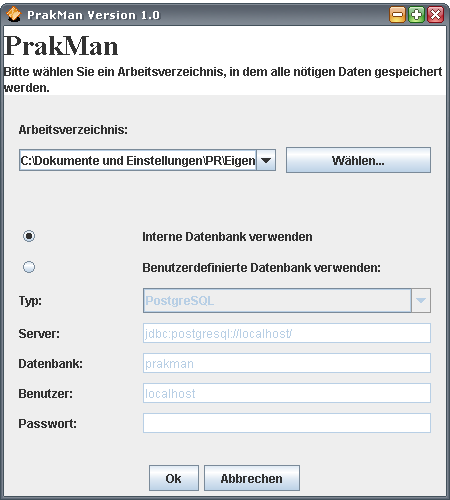
\includegraphics[scale=\screensize]{gfx/hb/hb_start}
\caption{Startbildschirm von ``PrakMan''}
\label{img:hb_start}
\end{center}
\end{figure}

\subsection{Hauptbildschirm}
\label{subsec:hb_hauptGUI}
Wurden alle Einstellungen im Startdialog gemacht und eine Verbindung zur gew�hlten Datenbank erfolgreich hergestellt, wird die in Abb.\ref{img:hb_hauptGui} (S.\pageref{img:hb_hauptGui}) dargestellte Oberfl�che aufgerufen. Dieses Fenster bleibt die ganze Zeit �ber sichtbar und ist in drei Bereiche aufgeteilt.

\begin{enumerate}
\item Die Men�leiste: Hier kann der Arbeitsbereich bzw. die Datenbank gewechselt sowie s�mtliche Studentendaten ausgedruckt werden. Auch Informationen �ber ``PrakMan'' sind von dort aus erreichbar.
\item Der Baum im linken Teil. Hier sind s�mtliche Informationen aus der Datenbank aufgelistet: Alle Veranstaltungen, Dozenten sowie Studenten. �ber einen Doppelklick k�nnen diese Objekte dann im rechten Teil des Fensters ge�ffnet werden.
\item Die Arbeitsfl�che im rechten Teil. Hier werden alle Objekte ge�ffnet, um ihre Informationen anzusehen oder zu editieren.
\end{enumerate}

Der Baum bietet zudem f�r die �ste Veranstaltungen, Lehrende und Studenten sowie die darin enthaltenen Objekte unterschiedliche Men�s (siehe Abbildung \ref{img:hb_tree}, S.\pageref{img:hb_tree}), mit denen Daten importiert, exportiert, gedruckt, bearbeitet oder gel�scht werden k�nnen.

\begin{figure}[hb]
\begin{center}
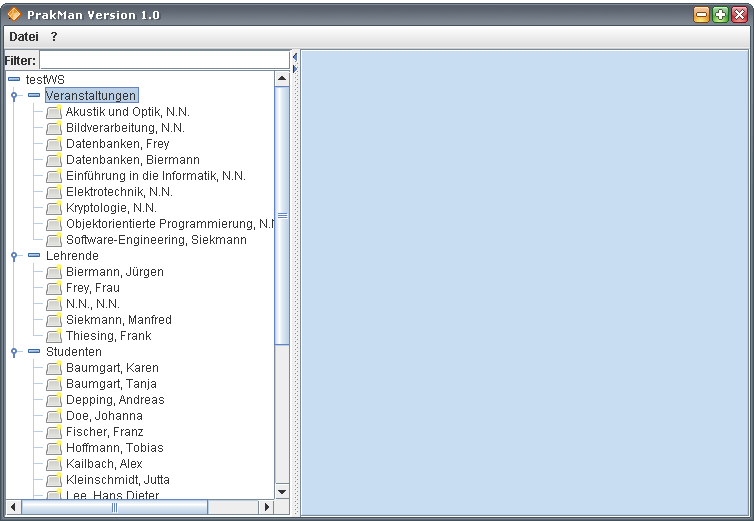
\includegraphics[scale=\screensize]{gfx/hb/hb_hauptGui}
\caption{Hauptbildschirm von ``PrakMan''}
\label{img:hb_hauptGui}
\end{center}
\end{figure}

\begin{figure}[hb]
\begin{center}
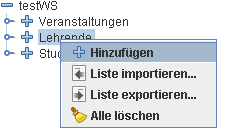
\includegraphics[scale=\screensize]{gfx/hb/hb_treeBranch}
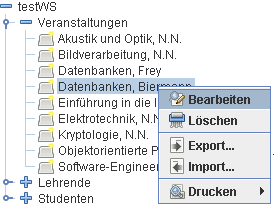
\includegraphics[scale=\screensize]{gfx/hb/hb_treeLeaf}
\caption{Men� eines Astes sowie eines Objekts im Dateibaum von ``PrakMan''}
\label{img:hb_tree}
\end{center}
\end{figure}

\subsection{Eine Veranstaltung: Teilnehmer}
\label{subsec:hb_eventTeilnehmer}
�ffnet der Benutzer per Doppelklick darauf (oder Rechtsklick, anschlie�end Bearbeiten) eine Veranstaltung, so �ffnet sich die in Abbildung \ref{img:hb_eventTeilnehmer} (S.\pageref{img:hb_eventTeilnehmer}) dargestellte Oberfl�che. Dort k�nnen �ber die Eingabefelder im oberen Bereich allgemeine Einstellungen der Veranstaltung ver�ndert werden: Der Name, der Dozent sowie die Beschreibung der Veranstaltung. Sollen diese Informationen gespeichert oder zur�ckgesetzt werden, helfen die Buttons ``Speichern'' und ``Zur�cksetzen'', die direkt dar�ber positioniert sind.

Die Tabelle darunter zeigt im standardm��ig ge�ffneten ``Teilnehmer-Tab'' die eingetragenen Teilnehmer der Veranstaltung samt Matrikelnummer, Nachname, Vorname und gegebenenfalls der bereits zugewiesenen Arbeitsgruppe.

Sollen genauere Infos �ber einzelne Studenten angezeigt werden, k�nnen diese mit einem einfachen Doppelklick ge�ffnet werden. Wenn Sie die Studenten in Gruppen einteilen m�chten, markieren Sie die gew�nschten Teilnehmer in der Tabelle (Shift und Strg-Tasten sind zur Unterst�tzung m�glich) und w�hlen Sie �ber einen Rechtsklick im darauf auftauchenden Men� die neue Gruppe aus.

Die vier Buttons im unteren Teil der Ansicht erm�glichen es, auf einen Schlag alle oder keinen Studenten zu markieren, sowie neue Teilnehmer hinzuzuf�gen oder alte zu entfernen.

\begin{figure}[hb]
\begin{center}
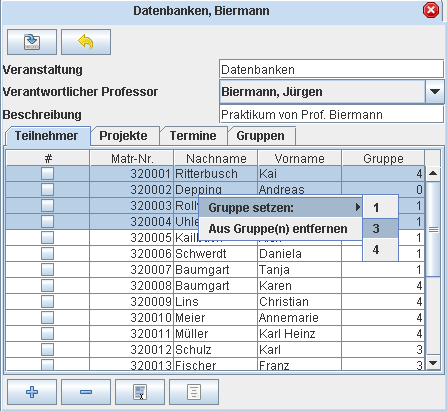
\includegraphics[scale=\screensize]{gfx/hb/hb_eventTeilnehmer}
\caption{Teilnehmeransicht einer Veranstaltung sowie Zuweisung einer Gruppe in ``PrakMan''}
\label{img:hb_eventTeilnehmer}
\end{center}
\end{figure}

\subsection{Eine Veranstaltung: Projekte}
\label{subsec:hb_eventProjekte}
Die in Abbildung \ref{img:hb_eventProjekte} (S.\pageref{img:hb_eventProjekte}) dargestellte Ansicht �ffnet sich, wenn beim Editieren eines Projektes (siehe Punkt \ref{subsec:hb_eventTeilnehmer}) der ``Projekte-Tab'' der Tabelle ausgew�hlt wird. Hier k�nnen alle f�r diese Veranstaltung angelegten Projekte eingesehen werden: Ihre Beschreibung, wann sie vergeben wurden und wann sie abgegeben werden soll(t)en.

Die vier Buttons am unteren Rand erm�glichen es nun, entweder alle oder kein Projekt anzuw�hlen sowie neue Projekte hinzuzuf�gen oder alte zu l�schen.

Ein Doppelklick auf ein existierendes Projekt �ffnet die in Abbildung \ref{img:hb_projektEdit} (S.\pageref{img:hb_projektEdit}) gezeigte Ansicht.
In dieser ist es m�glich, alle Daten eines Projektes zu �ndern: Die Beschreibung, Start- und Endtermin, sowie die Teilnehmer und deren Benotung.

Zum Editieren der Beschreibung, wird einfach eine neue in das entsprechende Textfeld eingetippt. Der ``Speichern-Button'' �bertr�gt die Informationen in die Datenbank. Zum Setzen des Start- und Endtermins m�ssen die Buttons am rechten Rand dieser Eingabezeilen genutzt werden. Diese �ffnen das in \ref{img:hb_datum} (S.\pageref{img:hb_datum}) gezeigte Fenster, in welchem eine Uhrzeit eingegeben sowie das gew�nschte Datum �ber die Oberfl�che ausgew�hlt werden kann. Die Studenten, die an diesem Projekt teilnehmen (sollen), k�nnen �ber die im unteren Teil implementierten ``Hinzuf�gen- und Entfernen-Buttons'' eingestellt werden. Zur Benotung eines einzelnen Studenten, reicht ein Doppelklick auf dessen Zeile in der Tabelle, welches das ebenfalls in Abbildung \ref{img:hb_projektEdit} (S.\pageref{img:hb_projektEdit}) gezeigte Eingabefeld �ffnet, �ber welches dann eine neue Note vergeben werden kann.

\begin{figure}[hb]
\begin{center}
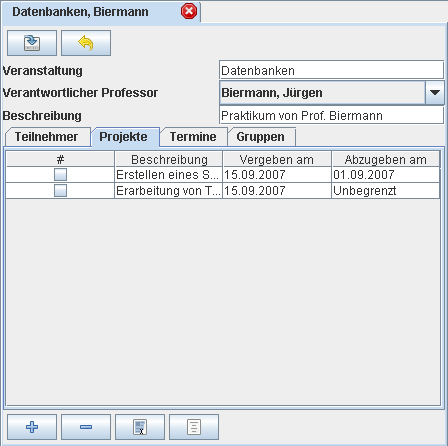
\includegraphics[scale=\screensize]{gfx/hb/hb_eventProjekte}
\caption{Projektansicht einer Veranstaltung in ``PrakMan''}
\label{img:hb_eventProjekte}
\end{center}
\end{figure}


\begin{figure}[hb]
\begin{center}
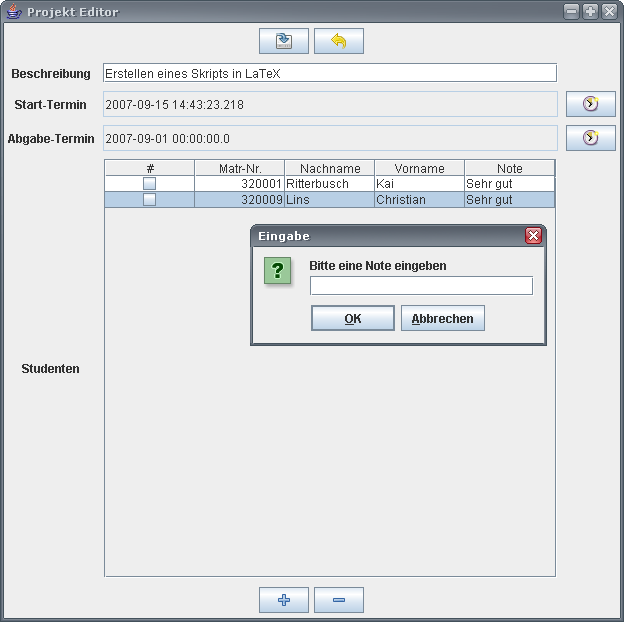
\includegraphics[scale=\screensize]{gfx/hb/hb_projektEdit}
\caption{Editieren eines Projektes sowie dessen Benotung in ``PrakMan''}
\label{img:hb_projektEdit}
\end{center}
\end{figure}

\begin{figure}[hb]
\begin{center}
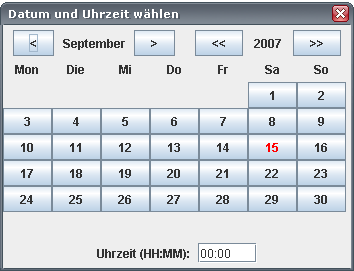
\includegraphics[scale=\screensize]{gfx/hb/hb_datum}
\caption{W�hlen eines Termins in ``PrakMan''}
\label{img:hb_datum}
\end{center}
\end{figure}

\subsection{Eine Veranstaltung: Termine}
\label{subsec:hb_eventTermine}
Die in Abbildung \ref{img:hb_eventTermine} (S.\pageref{img:hb_eventTermine}) dargestellte Ansicht �ffnet sich, wenn beim Editieren eines Projektes (siehe Punkt \ref{subsec:hb_eventTeilnehmer}) der ``Termine-Tab'' der Tabelle ausgew�hlt wird. Hier k�nnen alle f�r diese Veranstaltung angelegten Termine eingesehen sowie neue hinzugef�gt, alte gel�scht oder die tats�chlich anwesenden Teilnehmer eingetragen werden.


�ber die ``Hinzuf�gen- und Entfernen-Buttons'' am unteren Rand k�nnen nun neue Termine hinzugef�gt sowie in der Tabelle markierte Termine entfernt werden.
Soll ein neuer Termin angelegt werden, �ffnet sich das in Abbildung \ref{img:hb_eventTermine} (S.\pageref{img:hb_eventTermine}) gezeigte Fenster. Dort muss �ber den Datumsbutton ein Zeitpunkt gew�hlt werden. Anschlie�end kann �ber H�kchen in der darunter befindlichen Tabelle gew�hlt werden, welche Studenten anwesend waren. Die selbe Ansicht (mit den selben M�glichkeiten) �ffnet sich ebenfalls bei Doppelklick auf einen bereits vorhandenen Termin. Somit k�nnen auch alle Informationen im Nachhinein ge�ndert werden.

\begin{figure}[hb]
\begin{center}
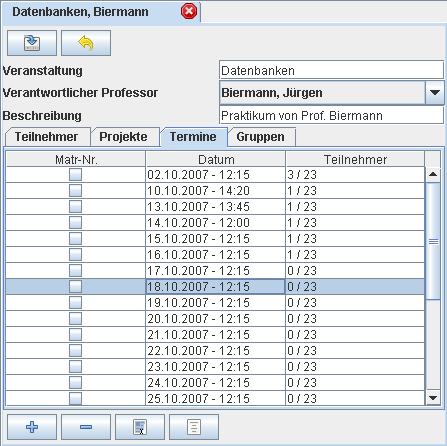
\includegraphics[scale=\screensize]{gfx/hb/hb_eventTermine}
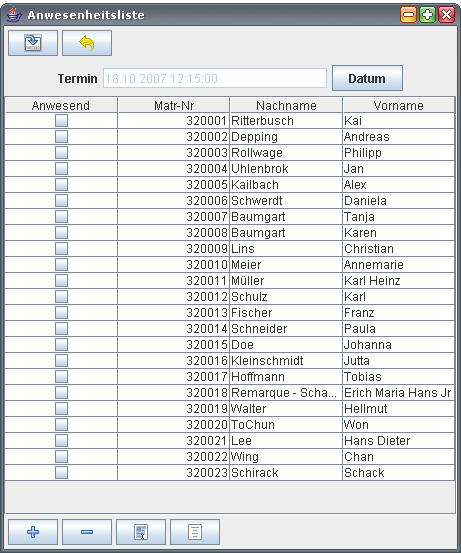
\includegraphics[scale=\screensize]{gfx/hb/hb_terminEdit}
\caption{Terminansicht einer Veranstaltung sowie Editieren eines Termins in ``PrakMan''}
\label{img:hb_eventTermine}
\end{center}
\end{figure}


\subsection{Eine Veranstaltung: Gruppen}
\label{subsec:hb_eventGruppen}
Die in Abbildung \ref{img:hb_eventGruppen} (S.\pageref{img:hb_eventGruppen}) dargestellte Ansicht �ffnet sich, wenn beim Editieren eines Projektes (siehe Punkt \ref{subsec:hb_eventTeilnehmer}) der ``Gruppen-Tab'' der Tabelle ausgew�hlt wird. Hier k�nnen alle f�r diese Veranstaltung angelegten Gruppen eingesehen sowie neue hinzugef�gt oder alte gel�scht werden.

Die Buttons unter der Tabelle erm�glichen es, von links nach rechts, eine neue Gruppe zu erstellen, eine markierte Gruppe zu l�schen, alle Gruppen zu selektieren und zuletzt alle abzuw�hlen.

Wird eine Gruppe �ber den ``Hinzuf�gen-Button'' erstellt, erscheint in der Tabelle eine neue Gruppe ohne Beschreibung. Diese kann dann noch, wie alle anderen Gruppen auch, �ber einen Doppelklick editiert werden. Dabei wird das in Abbildung \ref{img:hb_eventGruppen} (S.\pageref{img:hb_eventGruppen}) gezeigte Eingabefenster aufgerufen, in welchem die Beschreibung editiert und per Button gespeichert werden kann.

\begin{figure}[hb]
\begin{center}
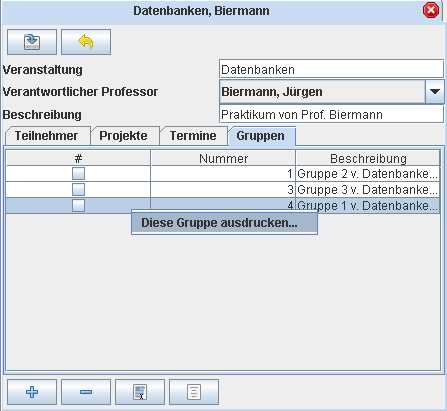
\includegraphics[scale=\screensize]{gfx/hb/hb_eventGruppen}
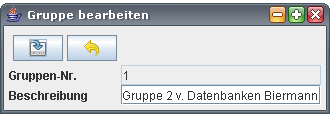
\includegraphics[scale=\screensize]{gfx/hb/hb_gruppeEdit}
\caption{Gruppenansicht einer Veranstaltung sowie Editieren von Gruppeninformationen in ``PrakMan''}
\label{img:hb_eventGruppen}
\end{center}
\end{figure}


\subsection{Ein Tutor: Betreute Veranstaltungen}
\label{subsec:hb_tutorPraktika}
�ffnet der Benutzer per Doppelklick darauf oder Rechtsklick > Bearbeiten einen Tutor, so �ffnet sich die in Abbildung \ref{img:hb_tutorPraktika} (S.\pageref{img:hb_tutorPraktika}) dargestellte Oberfl�che. Dort k�nnen �ber die Eingabefelder im oberen Bereich allgemeine Informationen �ber den Tutor editiert werden. Sollen diese Informationen gespeichert oder zur�ckgesetzt werden, helfen die Buttons ``Speichern'' und ``Zur�cksetzen'', die direkt dar�ber positioniert sind.

Die Tabelle im zentralen Bereich des Fensters listet alle Veranstaltungen auf, f�r die dieser Tutor als Betreuer eingesetzt ist. Ein Doppelklick auf eine Veranstaltung �ffnet diese in einem separaten Tab.

Die vier Buttons unter der Tabelle erm�glichen es, von links nach rechts, den Tutor f�r eine noch unbetreute Veranstaltung einzutragen, ihn von einer Veranstaltung als Tutor zu entfernen, alle Veranstaltungen zu w�hlen und schlie�lich alle abzuw�hlen.

\begin{figure}[hb]
\begin{center}
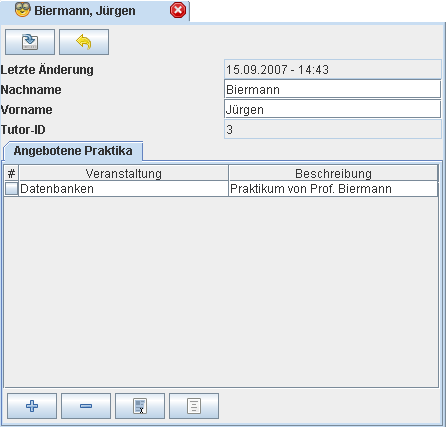
\includegraphics[scale=\screensize]{gfx/hb/hb_tutorPraktika}
\caption{Ansicht aller betreuten Veranstaltungen eines Tutors in ``PrakMan''}
\label{img:hb_tutorPraktika}
\end{center}
\end{figure}


\subsection{Ein Student: Gew�hlte Veranstaltungen}
\label{subsec:hb_studentPraktika}
�ffnet der Benutzer per Doppelklick darauf oder Rechtsklick > Bearbeiten einen Studenten, so �ffnet sich die in Abbildung \ref{img:hb_studentPraktika} (S.\pageref{img:hb_studentPraktika}) dargestellte Oberfl�che. Dort k�nnen �ber die Eingabefelder im oberen Bereich allgemeine Informationen �ber den Studenten editiert werden. Sollen diese Informationen gespeichert oder zur�ckgesetzt werden, helfen die Buttons ``Speichern'' und ``Zur�cksetzen'', die direkt dar�ber positioniert sind.

Die Tabelle im zentralen Bereich des Fensters listet alle Veranstaltungen auf, an denen dieser Student teilnimmt als auch, falls dies der Fall ist, die Arbeitsgruppe in der er sich befindet sowie deren Beschreibung. Ein Doppelklick auf eine Veranstaltung �ffnet diese in einem separaten Tab.

\begin{figure}[hb]
\begin{center}
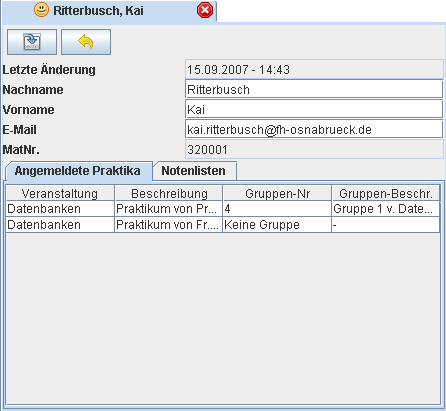
\includegraphics[scale=\screensize]{gfx/hb/hb_studentPraktika}
\caption{Ansicht aller gew�hlten Veranstaltungen eines Studenten in ``PrakMan''}
\label{img:hb_studentPraktika}
\end{center}
\end{figure}


\subsection{Ein Student: Noten}
\label{subsec:hb_studentNoten}
Die in Abbildung \ref{img:hb_studentNoten} (S.\pageref{img:hb_studentNoten}) dargestellte Ansicht �ffnet sich, wenn beim Editieren eines Projektes (siehe Punkt \ref{img:hb_studentPraktika}) der ``Noten-Tab'' der Tabelle ausgew�hlt wird. Hier k�nnen alle Noten eingesehen werden, die der Student bereits in jeglichen Veranstaltungen f�r unterschiedliche Projekte bekommen hat.

\begin{figure}[hb]
\begin{center}
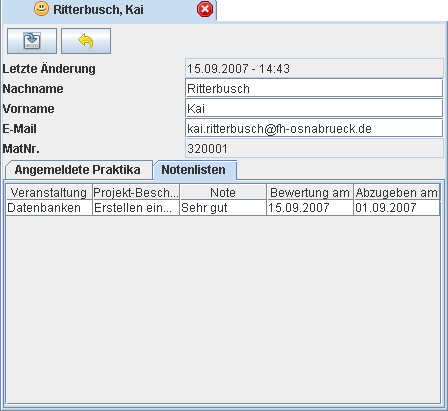
\includegraphics[scale=\screensize]{gfx/hb/hb_studentNoten}
\caption{Ansicht aller bisher erreichten Noten eines Studenten in ``PrakMan''}
\label{img:hb_studentNoten}
\end{center}
\end{figure}

% experimentell
\clearpage


\section{Datensicherung}
\label{sec:Datensicherung}
S�mtliche Daten von ``PrakMan'' sind in der Datenbank gesichert und werden von dieser verwaltet. Eine eigene Datensicherung ist somit nicht notwendig, da die unterst�tzten Datenbanken eigene Backup-Methoden anbieten, welche genutzt werden sollten. Der CSV-Export macht es zudem m�glich, manuell wichtige Daten zu extrahieren und eigenst�ndig zu sichern.

%\glossary{name={Event},description={Eine Veranstaltung oder ein Praktikum f�r eine gegebene Veranstaltung}}
%\glossary{name={Project},description={Eine Aufgabe, die an Studierende verteilt werden kann. Projekte sind notwendig, um Noten zu verteilen. Ein Projekt kann demnach auch das Bestehen der gesamten Veranstaltung darstellen.}}

\abbrev{Event}{Eine Veranstaltung oder ein Praktikum f�r eine gegebene Veranstaltung}

\abbrev{PrakMan}{Steht f�r Praktikums-Manager, das dokumentierte Programm.}

\abbrev{Project}{Eine Aufgabe, die an Studierende verteilt werden kann. Projekte sind notwendig, um Noten zu verteilen. Ein Projekt kann demnach auch das Bestehen der gesamten Veranstaltung darstellen.}

\abbrev{SubVersion (SVN)}{SubVersion ist eine Open-Source-Software zur Versionsverwaltung von Dateien und Verzeichnissen.}

%\chapter{Begriffserkl�rung}
\label{chap:Glossar}

\printnomenclature
\clearpage

% Nomenklatur erstellen:

% "c:\Programme\MiKTeX 2.5\miktex\bin\makeindex.exe" index.nlo -s nomencl.ist -o index.nls

% -------------------
% Damit das Glossar richtig erstellt wird, m�ssen folgende Befehle aufgerufen werden:
% 1. Latex-Konvertierung
% 2. C:\Dokumente und Einstellungen\PR\Desktop\SE-Hausarbeit\Doku\PrakMan_Doku>"c:\Programme\MiKTeX 2.5\miktex\bin\makeindex.exe" -s index.ist -t index.glg -o index.gls index.glo
% 3. Latex-Konvertierung




\end{document}
